%
% Master thesis template for Ghent University (2018)
%
%
%  !!!!!!!!!!!!!!!!!!!!!!!!!!!!!!!!!!!!!!!!!!!!!!!!!!!!!!!!!!!!
%  !!  MAKE SURE TO SET lualatex OR xelatex AS LATEX ENGINE  !!
%  !!!!!!!!!!!!!!!!!!!!!!!!!!!!!!!!!!!!!!!!!!!!!!!!!!!!!!!!!!!!
%  !! For overleaf:                                          !!
%  !!     1. click gear icon in top right                    !!
%  !!     2. select `lualatex` in "latex engine"             !!
%  !!     3. click "save project settings"                   !!
%  !!                                                        !!
%  !!!!!!!!!!!!!!!!!!!!!!!!!!!!!!!!!!!!!!!!!!!!!!!!!!!!!!!!!!!!
%
%
%  History
%    2014         Doctoral Thesis of Bruno Volckaert
%    2017         Adapted to master thesis by Jerico Moeyersons
%    2018         Cleanup by Merlijn Sebrechts
%
%  Latest version
%    https://github.com/galgalesh/masterproef-template
%
\documentclass[11pt,a4paper,twoside, openany]{book}
\usepackage[a4paper,includeheadfoot,margin=2.50cm]{geometry}

\setlength{\parindent}{0cm}           % indent of the first sentence of a paragraph
\setlength{\parskip}{1em}             % space between paragraphs
\renewcommand{\baselinestretch}{1.2}  % stretch horizontal space between everything

\usepackage{graphicx}
\graphicspath{{images/}}
\usepackage{pdfpages}
\usepackage{enumitem}
\usepackage{float}
\usepackage{caption}
\usepackage{subcaption}
\usepackage[toc,page]{appendix}
\usepackage[section]{placeins}
\makeatletter
\AtBeginDocument{%
	\expandafter\renewcommand\expandafter\subsection\expandafter{%
		\expandafter\@fb@secFB\subsection
	}%
}
\makeatother
\usepackage{svg}
\usepackage{amsmath}
\usepackage{graphicx}
\usepackage{epstopdf}
\epstopdfsetup{update} % only regenerate pdf files when eps file is newer

\usepackage[chapter]{minted}                           % for modern code highlighting
\newenvironment{code}{\captionsetup{type=listing}}{}   % To get multiline code fragments working: https://tex.stackexchange.com/a/53540/72273

\AtBeginEnvironment{minted}{\fontsize{10}{10}\selectfont}

\PassOptionsToPackage{hyphens}{url}
\usepackage{hyperref}
\usepackage{url}

\usepackage{quotchap}              % For the fancy quotes next to the chapter titles

\usepackage[numbers]{natbib}       % For bibliography; use numeric citations
\bibliographystyle{IEEEtran}
\usepackage[nottoc]{tocbibind}     % Put Bibliography in ToC

%
% Defines \checkmark to draw a checkmark
%
\usepackage{tikz}
\def\checkmark{\tikz\fill[scale=0.4](0,.35) -- (.25,0) -- (1,.7) -- (.25,.15) -- cycle;}

%
% For tables
%
\usepackage{booktabs}
\usepackage{array}
\usepackage{ragged2e}  % for '\RaggedRight' macro (allows hyphenation)
\newcolumntype{L}[1]{>{\raggedright\let\newline\\\arraybackslash\hspace{0pt}}m{#1}}
\newcolumntype{C}[1]{>{\centering\let\newline\\\arraybackslash\hspace{0pt}}m{#1}}
\newcolumntype{R}[1]{>{\raggedleft\let\newline\\\arraybackslash\hspace{0pt}}m{#1}}

%
% Support for splitting Dutch words correctly
%
\usepackage{polyglossia}
\setdefaultlanguage[babelshorthands=true]{dutch}

% Manually specify additional hypnations for words
\hyphenation{}

%
% Translated strings. If these aren't set, the English words are used.
%
\addto\captionsenglish{%
  \renewcommand{\contentsname}%
    {Inhoudsopgave}%
}
\renewcommand\appendixtocname{Bijlagen}
\renewcommand\appendixpagename{Bijlagen}
\renewcommand{\listoflistingscaption}{Lijst van listings}

\newfloat{code}{thp}{lop}
\floatname{code}{Code}

\newcommand\foreign[1]{\emph{#1}}
\newcommand\inlinecode[1]{\emph{#1}}
%
% Set the title and your name
%
\title{The user perceived performance of route planning APIs}
\author{Bert Marcelis}

%
%  END OF HEADER
%  The actual latex document content starts here.
%
\begin{document}

\includepdf{voorblad.pdf}             % Front matter
\newpage\thispagestyle{empty}\mbox{}  % White page
\thispagestyle{empty}    % Don't show page number

\begin{center}
\textbf{Dankwoord}



Na een intensieve periode van zes maanden is het zover. Met het schrijven van dit dankwoord leg ik de laatste hand aan mijn scriptie. Het was een periode waarin ik veel heb geleerd, op wetenschappelijk gebied, maar ook op persoonlijk vlak. Het schrijven van deze scriptie is me niet in de koude kleren gaan zitten. Ik wil graag stil staan bij de mensen die mij de afgelopen periode enorm hebben gesteund en geholpen.

Ik wil graag mijn collega’s van mijn stagebedrijf Central P. bedanken voor de fijne samenwerking. Jullie hebben mij enorm gesteund en waren altijd bereid om mij te helpen. Ik wil in het bijzonder stilstaan bij mijn begeleider bij Central P., mevrouw P. Buffay. Phoebe, ik wil je graag bedanken voor de fijne samenwerking en alle kansen die ik bij Central P. heb gekregen om mijn onderzoek uit te voeren en mijn scriptie te schrijven.

Daarnaast wil ik graag mijn studiebegeleiders, de heren C. Bing en R. Geller bedanken voor de fijne begeleiding. Jullie hebben mij de juiste handvatten aangereikt om de goede richting te kiezen, zodat ik mijn scriptie succesvol heb kunnen afronden.

Mijn ouders wil ik graag bedanken voor de wijze raad en luisterend oor. Jullie staan altijd voor mij klaar. Evenals mijn vrienden en vriendinnen. We konden altijd sparren over onze problemen, bevindingen, maar gelukkig ook over iets anders praten dan alleen die scriptie.

Lieve allemaal, heel erg bedankt!

\end{center}
          % Word of thanks
\newpage\thispagestyle{empty}\mbox{}  % White page
%\includepdf[pages={-}]{abstract.pdf}  % Extended Abstract
\tableofcontents                      % Table of Contents
\listoffigures                        % List of figures
\listoftables                         % List of tables
\listoflistings                       % List of listings (code fragments)

%
% Include the main chapters of the thesis below
%

% https://twitter.com/Stwaf/status/989531577947492358

\begin{savequote}[0.55\linewidth]
	``Inspirational quote''
	\qauthor{\textasciitilde Source}
\end{savequote}

\chapter{Inleiding}
\label{chap:intro}
Openbaar vervoer is een essentiële dienst in elke stad\citep{programmableweb14}. Om vlot van dit openbaar vervoer gebruik te maken, zijn er tientallen websites en apps (user-agents) die gebruikers informatie verstrekken over vertrekken, aankomsten, ritten, routes en vertragingen. Voorbeelden hiervan in België zijn iRail.be, HyperRail en Railer, en CityMapper, TheTransitApp, Here WeGo en Google maps wereldwijd. Op dit moment zijn al deze user-agents echter toegewezen op het gebruik van data dumps of specifieke APIs om informatie met betrekking tot openbaar vervoer te publiceren, of een variant ervan. 

Enerzijds zijn er volledige data dumps, in de vorm van General Transit Feed Specification (GTFS)\footnote{https://developers.google.com/transit/gtfs/} en General Transit Feed Specification Realtime (GTFS-RT)\footnote{https://developers.google.com/transit/gtfs-realtime/}. GTFS bestanden bevatten informatie over alle voertuigen van een dienstverlener, over een relatief grote tijdspanne, typisch enkele maanden tot een jaar. GTFS-RT bestanden bevatten realtime informatie over ritten in de komende dag. Om al deze data compact op te slaan en te versturen, worden deze opgeslagen in de vorm van regels. Deze regels omschrijven wanneer welk voertuig welke rit maakt. Om op basis van deze regels vragen te beantwoorden, dient deze set abstracte regels omgevormd te worden naar een gepast model waarin ritten en stopplaatsen opgevraagd kunnen worden, en routes berekend kunnen worden. Hiervoor zijn, afhankelijk van welke informatie gewenst is, zware berekeningen vereist, die afhankelijk van de grootte van het GTFS bestand vijf à tien minuten kunnen duren op een moderne computer. Gebruikers kunnen geen 10 minuten wachten tot de data getransformeerd zijn, waardoor deze optie niet beschikbaar is op mobiele toestellen. Verder is dit formaat een mogelijke technologische restrictie op de vervoersdata: enkel gevorderde ontwikkelaars kunnen hiervan gebruik maken. Open data is slechts open als deze (onder andere) beschikbaar zijn in een begrijpbaar formaat~\citep{okfn18}. GTFS is dus vooral geschikt om vervoersdata te delen met grote bedrijven, en in mindere mate voor individuele ontwikkelaars die vervoers data eenvoudig willen visualiseren (digital signage, routeplanner applicaties, websites, ...).

% TODO: source + license or redraw for consistent style
\begin{figure}
	\centering
	\includegraphics[width=0.5\textwidth]{GTFS_class_diagram.png}
		\caption[GTFS structuur]{De bestandsstructuur van GTFS data.}
	\label{fig:ldfAxis}
\end{figure}
% TODO: visueler maken wat GTFS juist is
 
Anderzijds zijn er traditionele Remote Procedure Call (RPC) zoals iRail\footnote{https://irail.be}, die beschikken over verschillende endpoints die specifieke vragen kunnen beantwoorden. Achterliggend kunnen zware berekeningen uitvoeren of grote databases raadplegen zonder dat de gebruiker hier nadeel van ondervindt. Deze antwoorden zijn rechtstreeks bruikbaar voor de client toepassing, maar bieden enkel een antwoord op één specifieke vraag. Een andere vraag, al dan niet door dezelfde client, vereist een nieuwe request naar de server, en zal een ander antwoord tot gevolg hebben. Elk verzoek naar de server vraagt relatief veel processortijd langs de serverkant. Een continue internetverbinding is dus vereist, en server-side is een potentieel grote en dure infrastructuur nodig om aan alle vragen te voldoen. Een ander belangrijk nadeel bij deze techniek is dat deze data moeilijk te combineren zijn met andere datasets. Een route plannen die gebruik maakt van meerdere openbaar vervoer aanbieders is enkel mogelijk als iemand een API aanbiedt die achterliggend door meerdere datasets zoekt. Simpelweg twee API's combineren is niet mogelijk.

% TODO: source + license or redraw for consistent style
\begin{figure}
	\centering
	\includegraphics[width=0.80\textwidth]{RPC_API.jpg}
	\caption[RPC structuur]{De werkwijze van een RPC API.}
	\label{fig:ldfAxis}
\end{figure}

Deze twee methodes zijn elkaars tegengestelde. Ontwikkelaars moeten kiezen voor data die compact maar complex, en slechts indirect bruikbaar is, of voor een vraag-antwoord systeem wat voor elke nieuwe vraag een nieuw verzoek naar een server moet maken. Aan de IDLab onderzoeksgroep aan UGent is onderzoek gedaan naar Linked Connections (LC)\footnote{https://linkedconnections.org}, een nieuw formaat dat een nieuw evenwicht tracht te vinden. Alle vertrekken van alle voertuigen worden in één chronologische lijst verzameld, waarbij de lijst kan opgevraagd worden volgens vaste tijdsintervallen met een grootteorde van enkele minuten. Hierdoor hoeft de server enkel deze lijst in fragmenten aan te bieden, waarbij alle clients dezelfde informatie krijgen. De clients dienen zelf nog berekeningen te maken, maar deze zijn relatief eenvoudig vergeleken met de berekeningen die nodig zijn om een GTFS feed te verwerken. Data in het Linked Connections formaat kunnen eenvoudig toegankelijk gemaakt worden via een open-source serverapplicatie\footnote{https://github.com/julianrojas87/linked-connections-server/}.

% TODO: betere kwaliteit, zie phd Pieter
\begin{figure}
	\centering
		\includegraphics[width=0.80\textwidth]{ldfAxis.png}
	\caption[Routeplanning HTTP interfaces op de LDF as]{De Linked Data Fragments as illustreert dat alle HTTP interfaces data fragmenten aanbieden, maar verschillen in hoe specifiek de aangeboden data is, en dus de moeilijkheid om deze aan te maken~\citep{verborgh14}. In deze figuur is de as toegepast op HTTP interfaces voor routeplanning~\citep{colpaert15}.}
	\label{fig:ldfAxis}
\end{figure}

\section{Wat is user-perceived performance?}
\label{sec:what_is_user_perceived_performance}
Elke interface voor het ophalen van data heeft specifieke eigenschappen zoals latency, performance, cache hergebruik,~...~\citep{verborgh16}. Wanneer we verschillende technieken vergelijken door dezelfde user-agent, kunnen we de impact van de verschillende achterliggende technieken op de eindgebruiker onderzoeken. Hiervoor definiëren we de user-perceived performance. De user-perceived performance is de performance zoals de gebruiker deze ervaart, welke niet strikt gelijk hoeft te zijn aan de performance van technische component. De user-perceived latency werd gedefinieerd in 2000 door Roy T. Fielding gedefinieerd als de tijd tussen het selecteren van een link en het renderen van een bruikbaar resultaat~\citep{fielding99}. Latency treedt op op verschillende punten: 
\begin{enumerate}
	\item de tijd die de client nodig heeft om actie te ondernemen 
	\item de tijd die nodig is voor voorbereidende acties
	\item de tijd om een verzoek te verzenden
	\item de tijd die de server nodig heeft om te antwoorden
	\item de tijd die nodig is om het antwoord te verzenden
	\item de tijd voor het antwoord te verwerken en weer te geven
\end{enumerate}
Terwijl enkel stappen 3, 4 en 5 rechtstreeks afhankelijk zijn van het netwerk, kunnen al deze stappen beïnvloed worden door de gebruikte techniek \citep{fielding99}.

Ondertussen zijn we geëvolueerd naar een wereld waarin data vaak mobiel geconsumeerd worden: 78\% van de Vlamingen beschikt over een smartphone, 80,5\% beschikt over een laptop. Slechts 41,8\% beschikt over een desktop-computer~\citep{digimeter17}. Hierbij zijn er ook andere aspecten die meespelen in de user experience: batterijgebruik en offline toegang tot data vormen een aanzienlijke factor in de user experience. Een applicatie presteert beter wanneer deze dezelfde data kan weergeven met aanzienlijk minder energieverbruik, of wanneer deze consistent goed presteert, ook wanneer netwerk slecht of niet beschikbaar is. Hoewel de user-perceived performance nog steeds gedomineerd wordt door de tijd tussen het selecteren van een link en het renderen van een bruikbaar resultaat, dienen we dus ook deze andere aspecten in rekening te brengen. Mobiele gebruikers hebben ook nog steeds angst om te veel data te verbruiken~\citep{ammelrooy17}.

% TODO: zal dit zo blijven of is er een trend ivm angst over datalimiet?

\section{Probleemstelling en doel van de masterproef}
\label{sec:problem}

Linked Connections werd ontwikkeld met de bedoeling een evenwicht te vinden tussen data dumps en RPC API's. In plaats van elke query op een server te beantwoorden, wordt een gelinkte lijst van connecties gepubliceerd. Linked Connections laat hierdoor toe om queries te beantwoorden door middel van een lineair groeiende lijst van connecties~\citep{colpaert15}. Bovendien gebruiken alle user-agents dezelfde lijst, waardoor deze zeer cachebaar is. Bij stijgende belasting daalt de tijd die nodig is per verzoek \citep{colpaert17}.

Terwijl de cost-efficiency van Linked Connections reeds is aangetoond, waarbij Linked Connections hetzelfde aantal verzoeken kan beantwoorden met slechts 25\% van de rekencapacteit\citep{colpaert17,Melendez17}, is er nog geen onderzoek gebeurt naar de user-perceived performance van een user-agent wanneer deze gebruik maakt van Linked Connections, vergeleken met wanneer deze zelfde user-agent gebruik maakt van een traditionele RPC API. 

In deze studie richten we ons specifiek op routeplanning gebruik makend van mobiele toestellen. Deze toestellen hebben minder processorkracht en geheugen vergeleken met traditionele computers, maar ook bandbreedte en beschikbaarheid van internet zijn vaak beperkt. In het slechtste geval is er geen netwerkverbinding, waarbij enkel een cache beschikbaar is. Verder zullen we ons specifiek richten op het verschil tussen een RPC API gebaseerd op Linked Connections~\citep{colpaert17} en de originele Linked Connections webserver. Als user-agent zullen we een fork van de Android HyperRail\footnote{https://hyperrail.be} applicatie gebruiken, gemodificeerd om de genoemde API's te gebruiken. Door deze testopstelling zijn de oorspronkelijke data, de server hardware, de user-agent en de client hardware gelijk bij elke vergelijking. Enkel het formaat voor serverinteracties en transport van data zal verschillen.

Om routes te berekenen zullen we gebruik maken van het Connection Scan Algorithm (CSA)~\citep{strasser13,strasser14,strasser17}. Dit algoritme vereist een op vertrektijd gesorteerde lijst van vertrekken. Dit is de exacte definitie van de LinkedConnections knowledge graph, waardoor dit algoritme zonder al te veel modificaties toegepast kan worden. Fragmenten kunnen hierbij geladen worden op het moment dat ze nodig zijn. We zullen dezelfde implementatie gebruiken zowel bij de client-side API als bij de server-side API om zo correct mogelijke resultaten te behalen. 

In eerste instantie zal een traditionele (RPC) API geschreven worden welke gebruik maakt van de Linked Connections fragmenten op de Solid State Disk (SSD) van de server. Deze API zal endpoints bevatten voor het tonen van vertrekken en aankomsten per station, het berekenen van routes, en voor het weergeven van het traject per trein. 
Vervolgens zal een API zonder specifieke server-side geïmplementeerd worden in de applicatie. Deze zal dezelfde informatie ter beschikking stellen in de applicatie, maar zal hiervoor enkel (delen van) de gelinkte lijst met vertrekken downloaden. 

Eenmaal beide API's volledig geïmplementeerd zijn, zal de user-experienced performance onderzocht worden. Hiertoe worden begeleide user tests gehouden, waarbij een aantal testgebruikers afwisselend met beide API's hun dagelijkse opzoekingen zullen uitvoeren, waarna ze aan de hand van een vragenlijst bevraagd zullen worden naar hun ervaringen en voorkeuren. Het is essentieel om de subjectieve ervaringen van gebruikers te bevragen, gezien verschillende gebruikers mogelijk verschillende afwegingen maken. We verwachten dat sommige gebruikers offline toegang waardevol zullen vinden, terwijl anderen mogelijk geen belang hechten aan offline toegang. Ook zal er technische data verzameld worden, zoals geheugen- en processorgebruik, laadtijden, en batterijverbruik. 

Deze masterproef zal gebruik maken van data afkomstig van de NMBS om routeplanning en realtime data over treinen in België weer te geven. Door de bron van de data te vervangen kan dit onderzoek ook toegepast worden op andere openbaar vervoer maatschappijen die gebruik maken van tijdsschema's, ongeacht het soort voertuig dat gebruikt wordt.

\section{Onderzoeksvraag}
 
 \paragraph{Onderzoeksvraag} Verbetert de user experience en user perceived perforance van een applicatie voor openbaar vervoer wanneer gebruik gemaakt wordt van Linked Connections in plaats van traditionele RPC API's?
 
 \paragraph{Hypothese 1} De gebruiker ervaart de mogelijkheid voor offline zoekopdrachten als een meerwaarde.
 
 \paragraph{Hypothese 2} De gebruiker ervaart de mogelijkheid om voorkeuren voor routes in te stellen (overstaptijd, toegankelijkheid, ...) als een meerwaarde.
 
\begin{savequote}[0.55\linewidth]
	``Inspirational quote''
	\qauthor{\textasciitilde Source}
\end{savequote}

\chapter{Implementatie}
Om een zo eerlijk mogelijke vergelijking te bekomen, zullen we zowel bij de client-side API als de server-side API dezelfde algorithmes toepassen. Gezien de jonge leeftijd van het Linked Connections framework zijn er nog geen algoritmes beschikbaar om deze data te verwerken. We zullen de ontwikkeling van deze algoritmen bespreken, met speciale aandacht voor het routeplanning algoritme vanwege de hogere complexiteit en de uitgebreide mogelijkheden.

\section{Linked Connections formaat}

In plaats van een dump van planningsdata of een volledige routeplanner te publiceren, publiceert Linked Connections paren van vertrek en aankomst voor elke treinrit, telkens van een station tot het volgende. Deze paren worden gesorteerd volgens vertrektijd. Hierna wordt deze lijst van paren gesplitst, om pagina's van gelijke grootte of gelijke tijdsduur te bekomen. Deze fragmenten kunnen gepubliceerd worden via HTTP als \foreign{JSON-LD}\footnote{https://json-ld.org/}, waarbij user-agents kunnen kiezen welke pagina's ze opvragen. Links in de gepubliceerde documenten zorgen ervoor dat user-agents steeds weten welke pagina ze als volgende moeten laden \citep{linkedconnections18}.

Om bovenstaande methode in de praktijk om te zetten, wordt gebruik gemaakt van de open source Linked-Connections-Server\footnote{https://github.com/julianrojas87/linked-connections-server/}. Om GTFS om te zetten naar Linked Connections, wordt er achterliggend gebruik gemaakt van de gtfs2lc tool\footnote{https://github.com/linkedconnections/gtfs2lc}.

Deze data is publiek toegankelijk via http://graph.irail.be/.

\subsection{Vraag- en antwoordformaat}
Om een pagina met data op te halen, wordt een verzoek gemaakt naar de API, waarbij de vervoersmaatschappij en het gewenste tijdstip in ISO8601 formaat in de URL opgenomen worden.  Codefragment \ref{code:linkedconnections-response} toont een ingekort resultaat voor de vertrekken bij de NMBS op 20 maart 2018, 12:30. De volledige specificatie\footnote{https://linkedconnections.org/specification/1-0} kan teruggevonden worden in \nameref{appendix:LinkedConnectionsSpec}.

Verzoek: \inlinecode{https://graph.irail.be/sncb/connections?departureTime=2018-03-20T12:30:00.000Z}

In dit codefragment vinden we volgende data terug:
\begin{enumerate}
	\item \foreign{@context}: Deze lijst definieert de gebruikte namespaces en velden
	\item \foreign{hydra:next} en  \foreign{hydra:previous}: Links naar de pagina met respectievelijk de volgende en de voorgaande data
	\item \foreign{hydra:search}: Informatie over de huidige pagina
	\item \foreign{@graph}: Deze lijst bevat de eigenlijke data. Elk vertrek bevat de volgende informatie:
	\begin{enumerate}
			\item \foreign{departureStop}: De URI welke het station van vertrek uniek identificeert.
			\item \foreign{arrivalStop}: De URI welke het station van aankomst uniek identificeert.	\item departureTime, arrivalTime: De geplande tijden, respectievelijk bij vertrek en aankomst.
			\item \foreign{departureDelay}, \foreign{arrivalDelay}: De vertraging, respectievelijk bij vertrek en aakomst.
			\item \foreign{direction}: De richting van dit voertuig, wat vaak ook op de lichtkrant van het voertuig weergegeven wordt.
			\item \foreign{gtfs:trip}: Een URI welk de rit van het voertuig uniek identificeert
			\item \foreign{gtfs:route}: Een URI welk de route van het voertuig uniek identificeert
			\item \foreign{gtfs:pickupType} en \foreign{gtfs:dropOffType}: geeft aan of reizigers al dan niet kunnen op- of afstappen bij respectievelijk vertrek en aankomst
	\end{enumerate}
\end{enumerate}

\begin{code}
	\begin{minted}[breaklines,tabsize=2]{json}

{
	"@context": {
	 "xsd": "http://www.w3.org/2001/XMLSchema#",
	"lc": "http://semweb.mmlab.be/ns/linkedconnections#",
	"hydra": "http://www.w3.org/ns/hydra/core#",
	"gtfs": "http://vocab.gtfs.org/terms#",
	"Connection": "lc:Connection",
	"...": "..."
	},
	"@id": "https://graph.irail.be/sncb/connections?departureTime=2018-03-20T12:30:00.000Z",
	"@type": "hydra:PagedCollection",
	"hydra:next": "https://graph.irail.be/sncb/connections?departureTime=2018-03-20T12:40:00.000Z",
	"hydra:previous": "https://graph.irail.be/sncb/connections?departureTime=2018-03-20T12:20:00.000Z",
	"hydra:search": {
		"..."
	},
	"@graph": [
		{
		"@id": "http://irail.be/connections/8822228/20180320/S11961",
		"@type": "Connection",
		"departureStop": "http://irail.be/stations/NMBS/008822228",
		"arrivalStop": "http://irail.be/stations/NMBS/008822210",
		"departureTime": "2018-03-20T12:30:00.000Z",
		"departureDelay": 60,
		"arrivalTime": "2018-03-20T12:32:00.000Z",
		"arrivalDelay": 0,
		"direction": "Anvers-Central",
		"gtfs:trip": "http://irail.be/vehicle/S11961/20180320",
		"gtfs:route": "http://irail.be/vehicle/S11961",
		"gtfs:pickupType": "gtfs:Regular",
		"gtfs:dropOffType": "gtfs:Regular"
		},
		{"...":"..."}
	]
}
	\end{minted}
\caption{Voorbeeld Linked Connections Formaat}
\label{code:linkedconnections-response}
\end{code}
\section{Connection Scan Algoritme}
Routeplanning wordt vaak opgelost met behulp van (een variant op) het algoritme van Dijkstra \citep{strasser13}. Toepassingen die gebruik maken van Dijkstra vereisen echter een graaf en een \foreign{priority queue}. Naast de impact op prestaties die deze eisen vormen, beperkt een graaf ook de flexibiliteit. De \foreign{open world assumption} stelt dat er steeds andere stopplaatsen wiens bestaan we (nog) niet kennen. Het opstellen van een graaf zou vereisen dat we alle gegevens eerst volledig moeten downloaden, terwijl Linked Connections net goed geschikt is voor streaming.


Het Connection Scan Algoritme (CSA) werd voor het eerst beschreven door Ben Strasser in 2013\citep{strasser13}. Dit algoritme vereist van een lijst met vertrekken gesorteerd op vertrektijd. Hiermee worden alle routes in een tijdsinterval efficiënt berekend\citep{strasser14,strasser17}. In tegenstelling tot Dijkstra's algoritme is er geen graaf of \foreign{priority queue} benodigd. Waar andere algoritmen ofwel enkel op kleine netwerken performant zijn, ofwel niet altijd de  best mogelijke route vinden, kan CSA de optimale route in grote netwerken toch efficiënt vinden\citep{strasser14}. In de praktijk is het vooral belangrijk om snel rekening te kunnen houden met vertragingen bij vertrek of aankomst\citep{strasser14,strasser17}. CSA berekent oorspronkelijk de snelste route, al is dit duidelijk niet altijd de route die de gebruiker wenst. Zo kan de snelste route nog steeds een station meermaals bezoeken, of kan men van een trein afstappen om later op deze zelfde trein weer op te stappen. Een oplossing hiervoor is om het aantal overstappen te beperken\citep{strasser14}.

Naast de tijd van aankomst, zijn er nog een aantal andere criteria die vaak geoptimaliseerd worden. Het populairste tweede criterium is het aantal overstappen, gevolgd door de prijs \citep{strasser17}. Optimalisatie van de prijs is echter zeer complex vanwege de complexe tariefplannen bij openbaar vervoer\citep{muller06}. Dit zullen we dan ook niet verder behandelen in dit onderzoek. 

\subsection{Implementatie en aanpassingen}
De werking en implementatie van CSA wordt behandeld in \citep{strasser17}. Dit algoritme kan zonder veel wijzigingen geïmplementeerd worden in zowel Java\footnote{https://github.com/Bertware/linkedconnections-android-client/blob/master/Hyperrail/src/main/java/be/hyperrail/android/irail/implementation/linkedconnections/RouteResponseListener.java} als PHP\footnote{https://github.com/hyperrail/lc2irail/blob/master/app/Http/Repositories/ConnectionsRepository.php}.

Wanneer dit algoritme geïmplementeerd wordt merken we echter duidelijke verschillen met de voorgestelde routes door de NMBS. Deze verschillen manifesteren zich vooral in de keuze van het station waar er overgestapt moet worden tussen twee treinen, en de keuze van de tussenliggende treinen indien er meer dan één overstap is. Zo is het mogelijk dat er wordt aangeraden om een trein te nemen langs Brussel Zuid en Centraal tot Noord, om van daar een andere trein te nemen die op zijn beurt van Brussel-Noord langs Centraal naar Zuid rijdt.
Verder zullen we ook nog aanpassingen doorvoeren om eenvoudig het aantal overstappen te beperken, en om op een betere manier aan \foreign{journey-extraction} te doen.

De implementatie en evolutie van het CSA algoritme worden uitgelegd aan de hand van code fragmenten in Java. Er wordt verondersteld dat sectie 4.2 van \cite{strasser17} gekend is. De code is asynchroon, waarbij na het laden van de eerste Linked Connections pagina een callback functie opgeroepen wordt om deze pagina te verwerken. Afhankelijk van het resultaat van deze verwerking, wordt er een nieuwe pagina opgevraagd, of wordt het resultaat doorgegeven aan de oproepende code door middel van callbacks.

Allereerst dienen we twee wijzigingen door te voeren aan de gegevensstructuren. De arrays S en T zijn vervangen door een Map, waardoor we onbeperkt nieuwe stations kunnen toevoegen. Dit maakt het algoritme geschikt om te werken rekening houdend met de open-world assumption. Voor een voertuig houden we niet enkel bij wanneer we zouden aankomen, maar ook met hoeveel overstappen (beginnend na het opstappen op deze trein) we zouden aankomen, en waar we moeten afstappen van deze trein. Dit laatste is essentieel om niet enkel de aankomsttijd, maar ook de exacte route met alle overstappen te kunnen weergeven. 

\begin{code}
	\begin{minted}[breaklines,tabsize=2]{java}
	class TrainTriple {
	/**
	* The arrival time at the final destination
	*/
	DateTime arrivalTime;
	
	/**
	* The number of transfers until the destination when hopping on to this train
	*/
	int transfers;
	
	/**
	* The arrival connection for the next transfer or arrival
	*/
	LinkedConnection arrivalConnection;
	}
	
	\end{minted}
\end{code}

Ook de paren van vertrek en aankomsttijd per station, zogehete profielen, worden aangepast. Naast de vertrek en aankomsttijd houden we nu ook de connectie bij waarmee we vertrekken in dit station op dit tijdstip, en de connectie waarmee we aankomen in het volgend station waar we moeten over- of afstappen. Ook het aantal overstappen, beginnend met tellen na het opstappen in dit station, wordt bijgehouden.

\begin{code}
\begin{minted}[breaklines,tabsize=2]{java}
  class StationQuadruple {
	/**
	* The departure time in this stop
	*/
	DateTime departureTime;
	
	/**
	* The arrival time at the final destination
	*/
	DateTime arrivalTime;
	
	/**
	* The departure connection in this stop
	*/
	LinkedConnection departureConnection;
	
	/**
	* The arrival connection for the next transfer or arrival
	*/
	LinkedConnection arrivalConnection;
	
	/**
	* The number of transfers between standing in this station and the destination
	*/
	int transfers;
}
	\end{minted}
\end{code}

Wanneer we de ingeladen connecties willen verwerken, filteren we alle connecties uit de pagina die ofwel te vroeg, ofwel te laat vallen. Ook moeten we een flag instellen wanneer we voorbij de vroegste vertrekdatum zijn. In dit geval zullen we na het overlopen van deze lijst geen nieuwe lijsten meer ophalen.

\begin{code}
\begin{minted}[breaklines,tabsize=2]{java}
	if (data.connections.length == 0) {
		mLinkedConnectionsProvider.getLinkedConnectionByUrl(data.previous, this, this, null);
		return;
	}
	
	boolean hasPassedDepartureLimit = false;
	for (int i = data.connections.length - 1; i >= 0; i--) {
		LinkedConnection connection = data.connections[i];
		
		if (connection.departureTime.isAfter(mArrivalLimit)) {
			continue;
		}
		if (connection.departureTime.isBefore(mDepartureLimit)) {
			hasPassedDepartureLimit = true;
			continue;
		}
		
		...
	}
	\end{minted}
\end{code}

Het bepalen van T1 en T2 spreekt voor zich, en loopt gelijk aan de implementatie uit \cite{strasser17}. In het geval dat er geen aankomst mogelijk is (binnen de beperkte tijd) stellen we zowel de aankomsttijd als het aantal overstappen in op een onrealistisch hoog getal. Dit vereenvoudigt de code aanzienlijk, aangezien er geen rekening gehouden hoeft te worden met het mogelijk leeg zijn van variabelen.
\begin{code}
	\begin{minted}[breaklines,tabsize=2]{java}
	 	if (Objects.equals(connection.arrivalStationUri, mRoutesRequest.getDestination().getSemanticId())) {
			T1_walkingArrivalTime = connection.arrivalTime;
			T1_transfers = 0;
		} else {
			T1_walkingArrivalTime = infinite;
			T1_transfers = 999;
		}

		// Determine T2, the first possible time of arrival when remaining seated
		if (T.containsKey(connection.trip)) {
			T2_stayOnTripArrivalTime = T.get(connection.trip).arrivalTime;
			T2_transfers = T.get(connection.trip).transfers;
		} else {
			T2_stayOnTripArrivalTime = infinite;
			T2_transfers = 999;
		}	
		\end{minted}
\end{code}

Bij de bepaling van T3 maken we de eerste grote afwijking van het oorspronkelijk algoritme. Om te bepalen of een overstap mogelijk is, moeten er reeds profielen voor dit station bekend zijn. Indien dit het geval is, gaan we op zoek naar het profiel waarbij er genoeg tijd is om over te stappen, maar waarbij het aantal overstappen het maximum aantal niet overschrijdt. 
Wanneer we een overstap vinden die aan deze voorwaarden voldoet, verhogen we het aantal overstappen ook met één. Deze aanpak is eenvoudiger dan de array-gebaseerde aanpak omschreven in \cite{strasser17}. Het voordeel van deze aanpak is dat automatisch alle snelste opties worden bijgehouden, zolang hun aantal overstappen onder het maximum blijft. 

In plaats van de door \cite{strasser17} voorgestelde verhoging van de aankomsttijd met één, om zo routes met een gelijke aankomsttijd maar minder overstappen voorkeur te geven, verhogen we hier de aankomsttijd met een vooraf gedefinieerd aantal seconden. Dit aantal geeft aan hoeveel seconden we langer op een trein wensen te zitten, in plaats van over te stappen. Door dit in te stellen op 240, wordt aangegeven dat een route die er tot 4 minuten langer over doet, met een overstap minder, toch de voorkeur krijgt over de snellere route met meer overstappen. Dit is een eerste veld wat door gebruikers ingesteld kan worden om de routes te personaliseren.

\begin{code}
	\begin{minted}[breaklines,tabsize=2]{java}
		// Determine T3, the time of arrival when taking the best possible transfer in this station
		if (S.containsKey(connection.arrivalStationUri)) {
			int position = S.get(connection.arrivalStationUri).size() - 1;
			StationQuadruple quadruple = S.get(connection.arrivalStationUri).get(position);
		
			while (
				(quadruple.departureTime.minusSeconds(transferSeconds).getMillis() <= connection.arrivalTime.getMillis() ||
				quadruple.transfers >= maxTransfers) &&  
				position > 0
			) {
				position--;
				quadruple = S.get(connection.arrivalStationUri).get(position);
			}
			if (quadruple.departureTime.minusSeconds(transferSeconds)
					.isAfter(connection.arrivalTime) && 
					quadruple.transfers <= maxTransfers) {
				T3_transferArrivalTime = quadruple.arrivalTime.plusSeconds(extraTimeInsteadOfTransfer);
				// Using this transfer will increase the number of transfers with 1
				T3_transfers = quadruple.transfers + 1;
			} else {
				// When there isn't a reachable connection, transferring isn't an option
				T3_transferArrivalTime = infinite;
				T3_transfers = 999;
			}
		} else {
			// When there isn't a reachable connection, transferring isn't an option
			T3_transferArrivalTime = infinite;
			T3_transfers = 999;
		}
		\end{minted}
\end{code}
Bij het bepalen van de vroegste aankomsttijd, wordt nu ook het aantal overstappen dat bij deze aankomsttijd hoort bepaald, en de connectie waar van de trein afgestapt wordt. We geven bij gelijke aankomsttijden de voorkeur aan overstappen: aangezien de vertrekkende voertuigen volgens dalende vertrektijd overlopen worden, geven we dus de voorkeur aan zo vroeg mogelijk overstappen. Dit geeft extra marge binnen de trip.
\begin{code}
\begin{minted}[breaklines,tabsize=2]{java}
DateTime Tmin;
LinkedConnection exitTrainConnection;
int numberOfTransfers;

if (T3_transferArrivalTime.getMillis() <= T2_stayOnTripArrivalTime.getMillis()) {
	Tmin = T3_transferArrivalTime;
	exitTrainConnection = connection;
	numberOfTransfers = T3_transfers;
} else {
	Tmin = T2_stayOnTripArrivalTime;
	if (T2_stayOnTripArrivalTime.isBefore(infinite)) {
		exitTrainConnection = T.get(connection.trip).arrivalConnection;
	} else {
		exitTrainConnection = null;
	}
	numberOfTransfers = T2_transfers;
}
// For equal times, we prefer just arriving.
if (T1_walkingArrivalTime.getMillis() <= Tmin.getMillis()) {
	Tmin = T1_walkingArrivalTime;
	exitTrainConnection = connection;
	numberOfTransfers = T1_transfers;
}

if (Tmin.isEqual(infinite)) {
	continue;
}
		\end{minted}
\end{code}
Door de extra toevoegingen voor journey extraction en het optimaliseren van de routes, is het bijwerken van de gegevenstructuren aanzienlijk ingewikkelder vergeleken met de originele implementatie. Voor voertuigen houden we niet langer enkel de aankomsttijd, maar ook de afstap halte bij. Hierbij verkiezen we de halte waarlangs we zo snel mogelijk aankomen, maar bij gelijke aankomsttijd wensen we een zo lang mogelijke periode voor de overstap. Wanneer de aankomsttijd gelijk is, onderzoeken we of de nieuwe afstap halte (de connectie die op dit moment onderzocht wordt) meer tijd voor een overstap geeft. Indien dit het geval is, werken we de afstap halte bij.
\begin{code}
	\begin{minted}[breaklines,tabsize=2]{java}
if (T.containsKey(connection.trip)) {

	if (Tmin.isEqual(T.get(connection.trip).arrivalTime) && 
		T3_transferArrivalTime.isEqual(T2_stayOnTripArrivalTime) &&
		S.containsKey(T.get(connection.trip).arrivalConnection.arrivalStationUri) &&
		S.containsKey(connection.arrivalStationUri)
	) {
		LinkedConnection currentTrainExit = T.get(connection.trip).arrivalConnection;
		
		StationQuadruple quad = new StationQuadruple();
		quad.departureTime = connection.departureTime;
		quad.departureConnection = connection;
		
		// Current situation
		quad.arrivalTime = Tmin;
		quad.arrivalConnection = currentTrainExit;
		Duration currentTransfer = new Duration(currentTrainExit.arrivalTime, getFirstReachableConnection(quad).departureTime);
		
		// New situation
		quad.arrivalTime = Tmin;
		quad.arrivalConnection = exitTrainConnection;
		Duration newTransfer = new Duration(exitTrainConnection.arrivalTime, getFirstReachableConnection(quad).departureTime);

		if (newTransfer.isLongerThan(currentTransfer)) {
			TrainTriple triple = new TrainTriple();
			triple.arrivalTime = Tmin;
			triple.arrivalConnection = exitTrainConnection;
			triple.transfers = numberOfTransfers;
			T.put(connection.trip, triple);
		}
	}
	
	if (Tmin.isBefore(T.get(connection.trip).arrivalTime)) {
		TrainTriple triple = new TrainTriple();
		triple.arrivalTime = Tmin;
		triple.arrivalConnection = exitTrainConnection;
		triple.transfers = numberOfTransfers;
		
		T.put(connection.trip, triple);
	}
} else {
	TrainTriple triple = new TrainTriple();
	triple.arrivalTime = Tmin;
	triple.arrivalConnection = exitTrainConnection;
	triple.transfers = numberOfTransfers;
	T.put(connection.trip, triple);
}

\end{minted}
\end{code}

De stopprofielen zijn lichtjes aangepast om de efficientie te verhogen. De vroegste vertrekken worden nu achteraan toegevoegd. Door deze aanpassing, en het gegeven dat de vertrektijd van de huidige connectie gelijk of kleiner dan de vertrektijd van alle vorige connecties is, hoeven we nu enkel het laatste profiel in de lijst te evalueren. Als de vertrektijd kleiner of gelijk is, moet de aankomsttijd kleiner zijn. we controleren dus enkel of de aankomsttijd kleiner is, en zo ja, of de vertrektijd kleiner of gelijk is. Afhankelijk van deze laatste controle voegen we een nieuw item toe aan de lijst, of vervangen we het laatste. Aangezien we telkens enkel toevoegen wanneer de aankomsttijd vroeger ligt, zal deze lijst altijd gesorteerd zijn volgens dalende aankomsttijd. Hiermee is bewezen dat deze optimalisatie correct is, en een beter alternatief voor het overlopen van de volledige lijst.L

\begin{code}
	\begin{minted}[breaklines,tabsize=2]{java}
StationQuadruple quad = new StationQuadruple();
quad.departureTime = connection.departureTime;
quad.arrivalTime = Tmin;

// Additional data for journey extraction
quad.departureConnection = connection;
quad.arrivalConnection = T.get(connection.trip).arrivalConnection;
quad.transfers = numberOfTransfers;

if (S.containsKey(connection.departureStationUri)) {
	int numberOfPairs = S.get(connection.departureStationUri).size();
	StationQuadruple existingQuad = S.get(connection.departureStationUri).get(numberOfPairs - 1);
	if (quad.arrivalTime.isBefore(existingQuad.arrivalTime)) {
		if (quad.departureTime.isEqual(existingQuad.departureTime)) {
			S.get(connection.departureStationUri).remove(numberOfPairs - 1);
			S.get(connection.departureStationUri).add(numberOfPairs - 1, quad);
		} else {
			S.get(connection.departureStationUri).add(quad);
		}
	}
} else {
	S.put(connection.departureStationUri, new ArrayList<StationQuadruple>());
	S.get(connection.departureStationUri).add(quad);
}
		\end{minted}
\end{code}
De lijst met volledige routes reconstrueren is relatief eenvoudig. Voor elk profiel horend bij de stoplocatie van waar de reiziger vertrekt, volgen we de vertrek- en aankomstconnecties. Om bij elke tussenstop de juiste connectie te vinden waarmee de reis verder zal gezet worden, vergelijken we de aankomsttijd uit het stopprofiel waaruit we vertrokken, met de aankomsttijden uit de stopprofielen van de tussenstop. Wanneer deze gelijk zijn, hebben we het volgende deel van de reis gevonden.
\begin{code}
\begin{minted}[breaklines,tabsize=2]{java}
// Results? Return data
Route[] routes = new Route[S.get(mRoutesRequest.getOrigin().getSemanticId()).size()];

int i = 0;
for (StationQuadruple quad : S.get(mRoutesRequest.getOrigin().getSemanticId())
) {
	// it will iterate over all legs
	StationQuadruple it = quad;
	List<RouteLeg> legs = new ArrayList<>();
	
	while (!Objects.equals(it.arrivalConnection.arrivalStationUri, mRoutesRequest.getDestination().getSemanticId())) {
		// use it.departureConnection and it.arrivalConnection to construct legs of this journey
		legs.add(...);
		it = getFirstReachableConnection(it);
	}
	
	routes[i++] = new Route(legs);
}
\end{minted}
\end{code}
\begin{code}
	\begin{minted}[breaklines,tabsize=2]{java}
private StationQuadruple getFirstReachableConnection(StationQuadruple arrivalQuad) {
	List<StationQuadruple> it_options = S.get(arrivalQuad.arrivalConnection.arrivalStationUri);
	int i = it_options.size() - 1;
		while (i >= 0 && it_options.get(i).arrivalTime.getMillis() != arrivalQuad.arrivalTime.getMillis() - 240 * 1000) {
		i--;
	}
	return it_options.get(i);
}
		\end{minted}
\end{code}

\section{Vertrekken en aankomsten per station}

\section{Route van een trein}
% !TeX spellcheck = nl_NL
\begin{savequote}[0.55\linewidth]
	``Inspirational quote''
	\qauthor{\textasciitilde Source}
\end{savequote}

\chapter{Onderzoek}
Gezien Linked Connections nog enkele belangrijke gegevens mist, zoals of een stop al dan niet afgeschaft is, en aan welk perron het voertuig zal aankomen of vertrekken, kunnen we dit systeem nog niet op grote schaal testen. In plaats hiervan zullen we beide implementaties testen in een gesloten omgeving om de objectieve verschillen te meten. Ook zullen we user-tests uitvoeren met gebruikers, waarbij gebruikers gevraagd wordt om hun gebruikelijke opzoekingen te doen, per implementatie hun mening te geven, en vervolgens te bevragen welke variant hun voorkeur geniet.

Om te voorkomen dat de keuze van het geteste station of route de objectieve metingen vertekent, zullen we de opzoekingen van echte gebruikers gebruiken. Hiervoor gebruiken we de log data van api.irail.be, die publiek beschikbaar is\footnote{https://gtfs.irail.be/logs}. Door deze queries opnieuw af te spelen op de applicaties kunnen we een zo goed mogelijk beeld krijgen van de werkelijke prestaties.

Objectief zullen we proberen om volgende gegevens vast te leggen
\begin{itemize}
	\item de tijd om alle data van de server te halen
	\item de tijd tussen zoekopdracht en weergave van het eerste resultaat
	\item de tijd tussen zoekopdracht en weergave van het volledig resultaat
	\item het processorgebruik van het toestel
	\item het batterijgebruik van het toestel
\end{itemize}
% !TeX spellcheck = nl_NL
\begin{savequote}[0.55\linewidth]
	``Inspirational quote''
	\qauthor{\textasciitilde Source}
\end{savequote}

\chapter{Resultaten}
\label{chap:resultaten}

Om te voorkomen dat de keuze van het geteste station of route de objectieve metingen vertekent, werden de opzoekingen van echte gebruikers gebruikt op 2 mei 2018\footnote{https://gtfs.irail.be/logs}. Om de duur van de testen enigszins binnen de perken te houden, worden niet alle opzoekingen getest, maar telkens een willekeurig gekozen selectie. Deze selectie werd gemaakt door uit de chronologische logboeken met zoekopdrachten telkens de n-de zoekopdracht te gebruiken.

Voor de alle tests werd gebruik gemaakt van een HTC 10 of HTC One, verbonden met internet via wifi (ping 26ms, downloadsnelheid 42mbps, uploadsnelheid 9mbps), tenzij anders vermeld. Het toestel werd niet gebruikt tijdens de testen, en er werden geen achtergrondapplicaties uitgevoerd. De metingen werden automatisch uitgevoerd met behulp van \foreign{instrumented tests}. Metingen van Linked Connections (LC) gebruiken de LoganSquare JSON parser.

De HTC 10 is een \foreign{flagship} smartphone, uitgebracht in maart 2016. Deze beschikt over een krachtige Snapdragon 820 processor en 4GB ram. De HTC One daarintegen is een \foreign{flagship} smartphone uit 2013, welke over een oude Snapdragon 800 processor en 2GB ram beschikt. Het HTC 10 toestel komt overeen met moderne toestel bovenaan in het mid-range aanbod. Dit toestel biedt goede prestaties en zullen we gebruiken om de performantie van Linked Connections op toestellen van 400 a 600 euro te testen. De HTC One komt op vlak van prestaties overeen met low-end toestellen en oudere mid-range toestellen, en komt ongeveer overeen met de prestaties van een paar jaar oude smartphone van 200 euro. Op deze manier krijgen we een indicatie van de performantie voor alle smartphonegebruikers.

% TODO: afbeelding met schaal?

\section{Liveboards}
\subsection{Metingen}
\begin{figure}[h]
	\centering
	\includegraphics[width=0.80\textwidth]{Optimalisaties_liveboards.eps}
		\caption[Gemeten laadtijd liveboards]{De gemeten laadtijd voor liveboards gebruikmakend van een HTC 10 voor 262 opzoekingen gebaseerd op de iRail logs. }
	\label{fig:liveboardlabtest}
\end{figure}
\begin{table}[h]
	\begin{tabular}{| c | c | c | c | c | c |}
		\hline
		Variant & parser & cache & minimaal (ms) & gemiddelde (ms) & maximaal (ms)\\
		\hline
		LC op toestel & org.json & nee & 302 &  595 &  3471 \\
		LC op toestel & org.json & ja & 409 &  516  &  3599 \\
		LC op toestel & LoganSquare & nee & 392 & 597 & 2027 \\
		LC op toestel & LoganSquare & ja  & 166 & 313 & 3428 \\
		
		LC op server &&&  232 & 397 &  1421\\
		\hline
	\end{tabular}
	\caption[Gemeten laadtijd liveboards]{De gemeten laadtijd voor het eerste resultaat liveboards gebruikmakend van een HTC 10 voor 262 opzoekingen gebaseerd op de iRail logs. }
	\label{tab:liveboardlabtest}
\end{table}

In tabel \ref{tab:liveboardlabtest} en grafiek \ref{fig:liveboardlabtest} zijn de resultaten zichtbaar van een benchmark waarbij 262 stations opgezocht werden, ongeveer 5\% van de opzoekingen door gebruikers op 2 mei 2018. Telkens is de minimale, gemiddelde en maximale responstijd gemeten. Dit zowel gebruikmakend van de standaard JSON parser (\foreign{org.json}) en gebruikmakend van de \foreign{LoganSquare} parser. Ook werd de test herhaald met cache in- en uitgeschakeld, om zo het effect hiervan te meten. Tot slot werd dezelfde test herhaald gebruikmakend van data afkomstig van de LC2Irail web applicatie om een vergelijking tussen de twee methodes te kunnen maken. Deze cijfers geven slechts een indicatie van de snelheid - een volledige en diepgaande statistische analyse van de performantieverschillen tussen verschillende implementatiedetails van dezelfde techniek valt wegens tijdsgebrek buiten het bereik van deze masterproef.

In deze cijfers is invloed van de cache wel duidelijk merkbaar. We zien wel een duidelijk verschil tussen de parsers: terwijl bij gebruik van de \foreign{LoganSquare} parser de gemiddelde laadtijd bijna halveert, terwijl het effect van de cache bij het gebruik van de \foreign{org.json} parser veel kleiner is. Wanneer de cache uitgeschakeld is is het verschil tussen de parsers verwaarloosbaar. Dit is te verklaren door het feit dat voor het tonen van vertrekken of aankomsten relatief weinig data nodig is: in de meeste gevallen volstaat een enkele Linked Connections pagina.

Om een exact beeld te vormen van de prestaties, zoeken we een duizendtal liveboards op. Hiervoor kiezen we telkens de vijfde opzoeking uit de iRail logs. Voor elk liveboard worden twintig resultaten geladen. De resultaten hiervan zijn zichtbaar in grafieken \ref{fig:liveboardsDiefBest}, \ref{fig:liveboardsDiefAvg} en \ref{fig:liveboardsDiefSlechtst}, respectievelijk voor het tiende, vijftigste en negentigste percentiel. Uit deze grafieken kunnen we duidelijke trends zien:
\begin{itemize}
\item In de snelste gevallen is de serverimplementatie sneller. Hiervoor kunnen we verschillende oorzaken aanwijzen: 
	\begin{itemize}
		\item De serverimplementatie kan resultaten op een specifieke vraag cachen, terwijl de lokale implementatie deze steeds zal herberekenen vanaf Linked Connections pagina's.
		\item De serverimplementatie hoeft minder data te versturen. Ook het parsen van het antwoord gaat sneller, gezien slechts een kleine hoeveelheid data verwerkt moet worden en er verder geen berekeningen moeten gebeuren.
	\end{itemize}
	\item Terwijl in de snelste gevallen de serverimplementatie sneller is, is dit verschil beperkt tot ongeveer 60 milliseconden voor het eerste resultaat. Dit is in praktijk amper merkbaar voor gebruikers %TODO: citation needed
	\item Wanneer we naar de mediane performantie kijken, is Linked Connections duidelijk sneller voor de eerste resultaten. Dit snelheidsverschil is aanzienlijk, en vooral te wijten aan het feit dat Linked Connections volledige ondersteuning biedt voor incrementele resultaten, waarbij de server steeds meerdere pagina's zal overlopen voor een antwoord gegeven wordt; Naarmate meer resultaten geladen worden, vormt het overlopen van meerdere pagina's een voordeel voor de serverimplementatie: Zo zullen in daluren sneller resultaten geladen worden door de snellere toegang tot Linked Connections pagina's, terwijl bij Linked Connections sprake is van een \foreign{overhead} door het laden van te veel data. Hierbij zien we dat hoe sneller het toestel, hoe langer Linked Connections het snelst blijft. Ook blijft het verschil tussen Linked Connections en LC2Irail beperkt op de HTC 10, terwijl dit verschil aanzienlijk oploopt op de HTC One.
	\item In alle gevallen is er een sterke gelijkenis tussen de curves voor LC2Irail op het HTC 10 toestel en het HTC One toestel. Deze zijn enkel een relatief kleine afstand in tijd verschoven, wat verklaart kan worden door de lage belasting voor het mobiele toestel wanneer een RPC API gebruikt wordt.
	\item Het verschil in laadtijd tussen Linked Connections op de twee toestellen loopt lineair op met de benodigde laadtijd om resultaten te laden. Zo zien we dat in het slechtste geval dubbel zoveel tijd benodigd is op de HTC One in vergelijking met de HTC 10.
\end{itemize}

\begin{figure}[h]
	\centering
	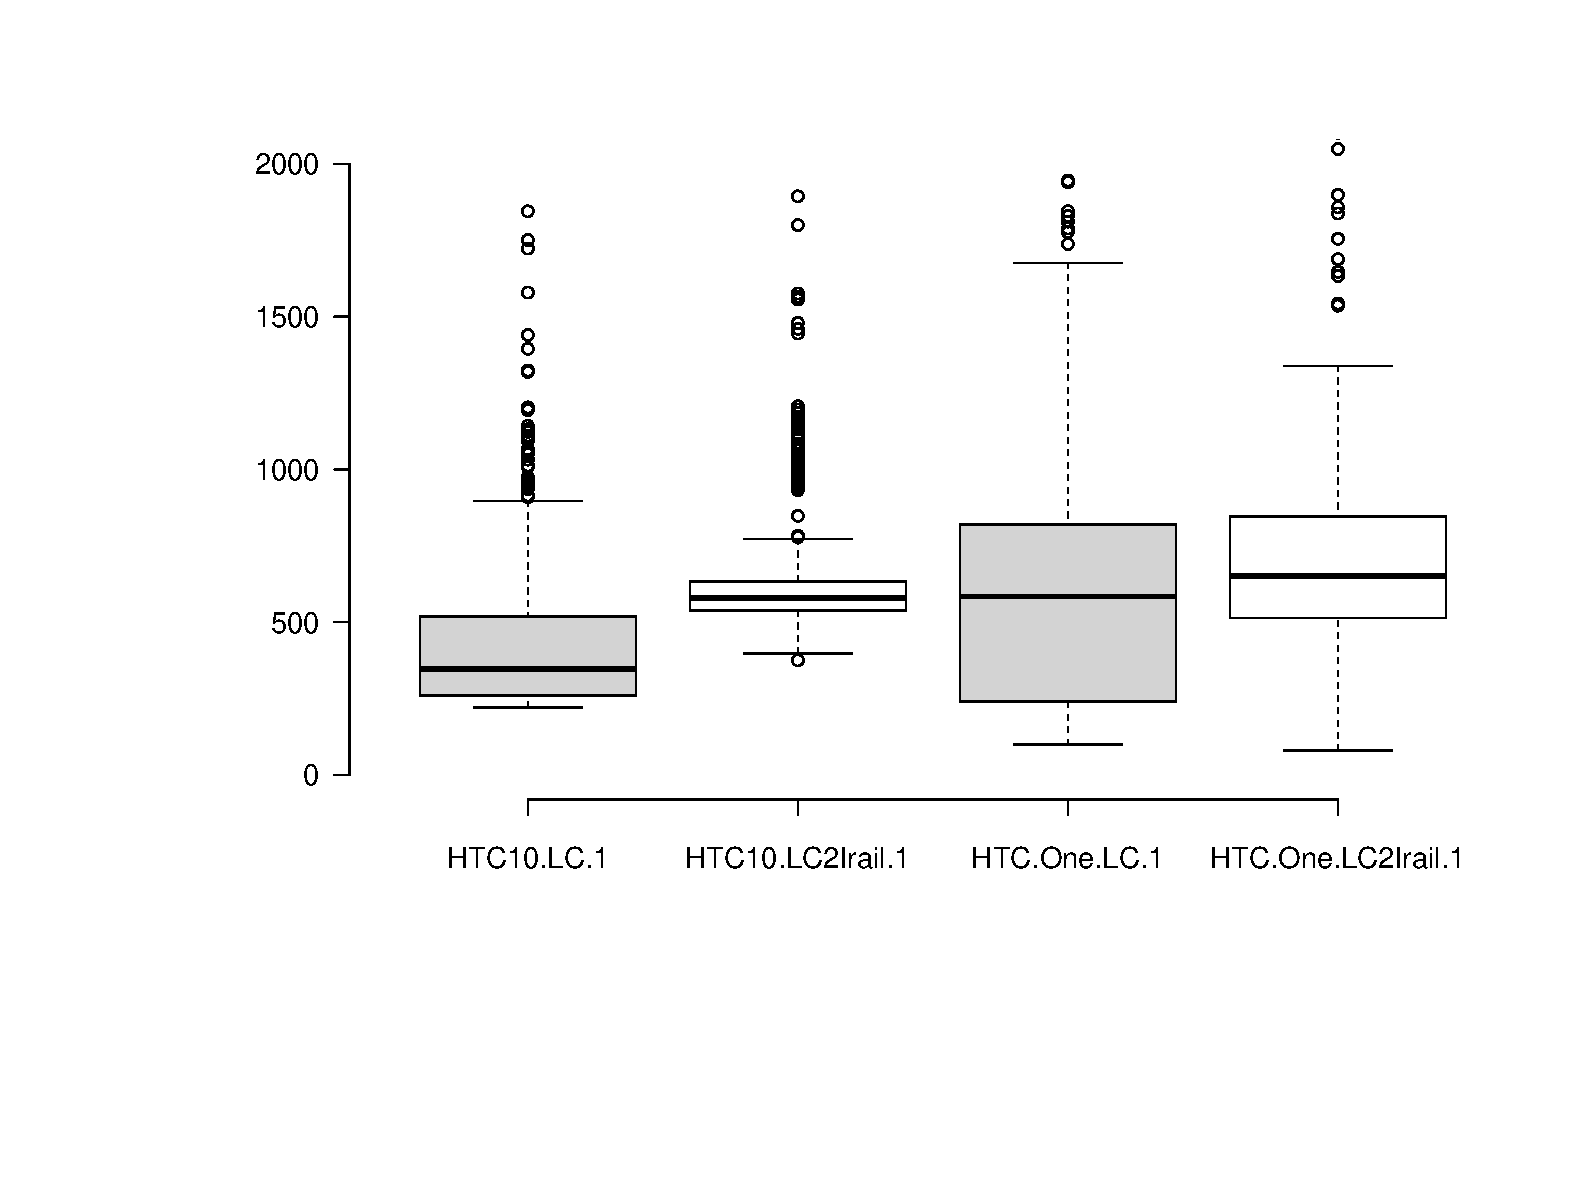
\includegraphics[width=1.00\textwidth]{boxplot_liveboards_1.eps}
	\caption[Laadtijd eerste resultaat liveboard in functie van toestel en technologie]{Laadtijd eerste resultaat liveboard in functie van toestel en technologie.}
	\label{fig:liveboardsBoxplot1}
\end{figure}

\begin{figure}[h]
	\centering
	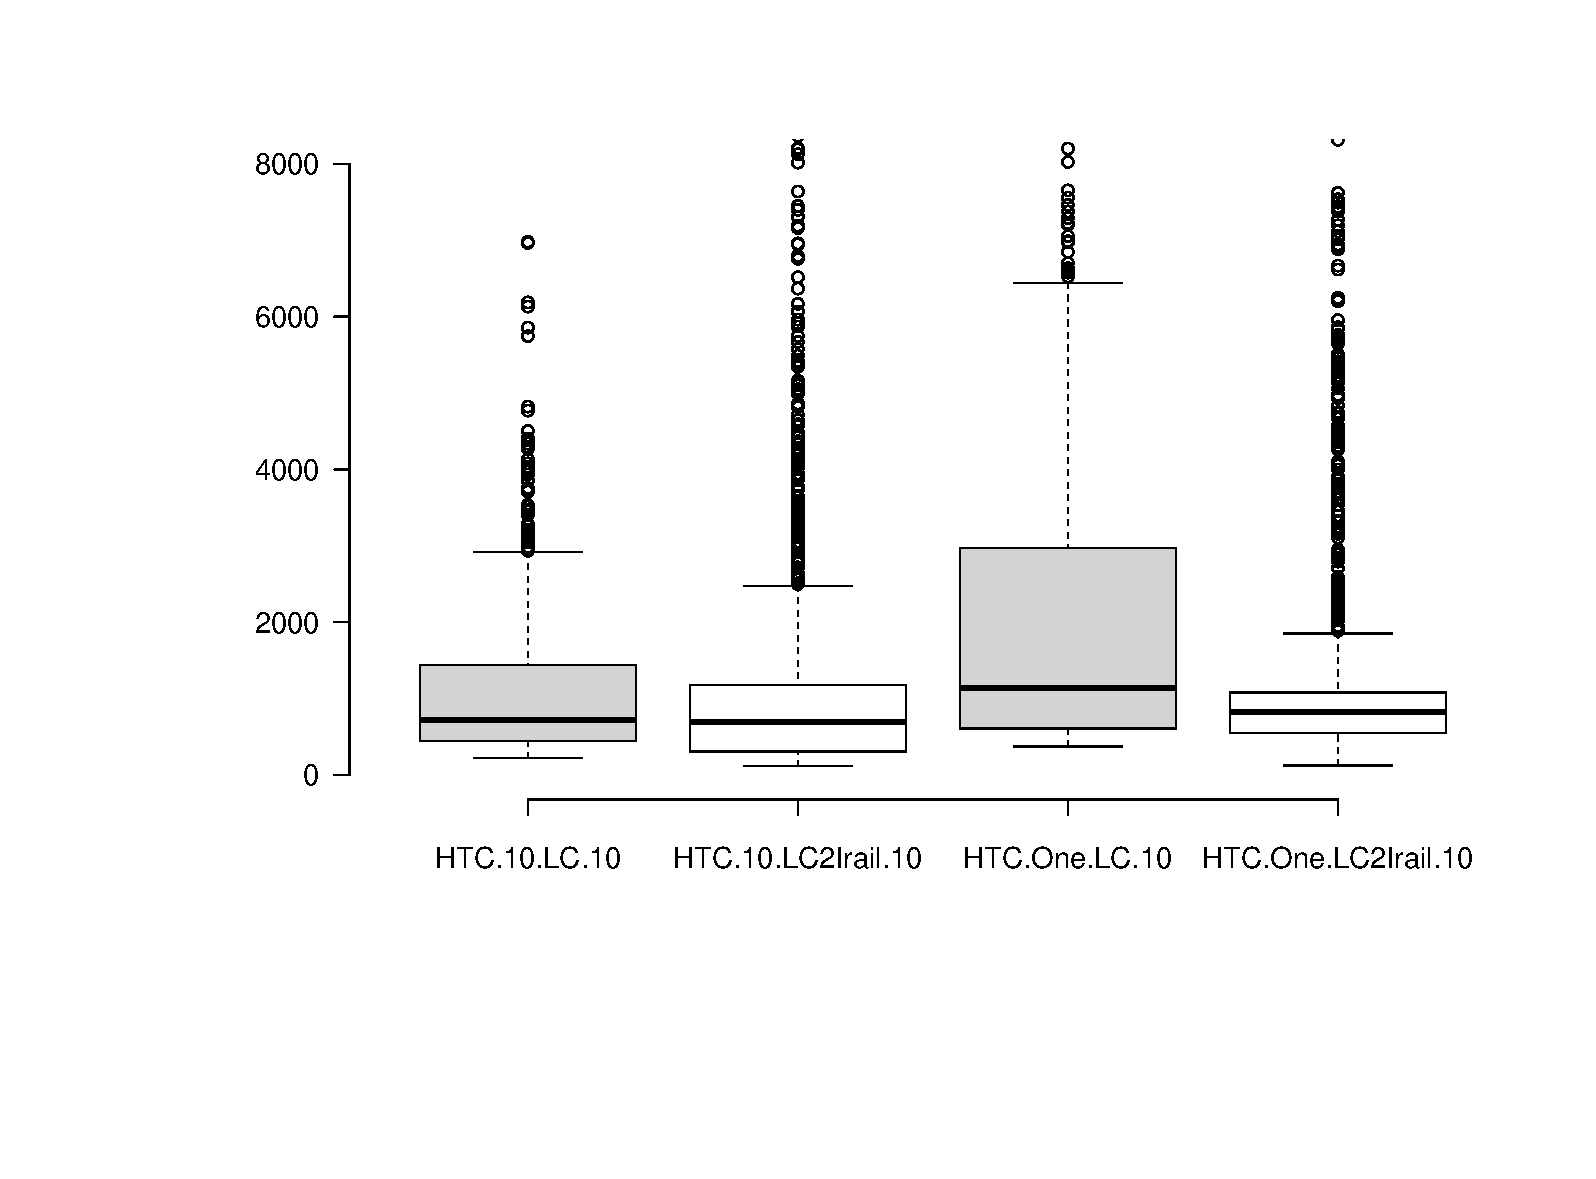
\includegraphics[width=1.00\textwidth]{boxplot_liveboards_10.eps}
	\caption[Laadtijd tiende resultaat liveboard in functie van toestel en technologie]{Laadtijd tiende resultaat liveboard in functie van toestel en technologie.}
	\label{fig:liveboardsBoxplot10}
\end{figure}

\begin{figure}[h]
	\centering
	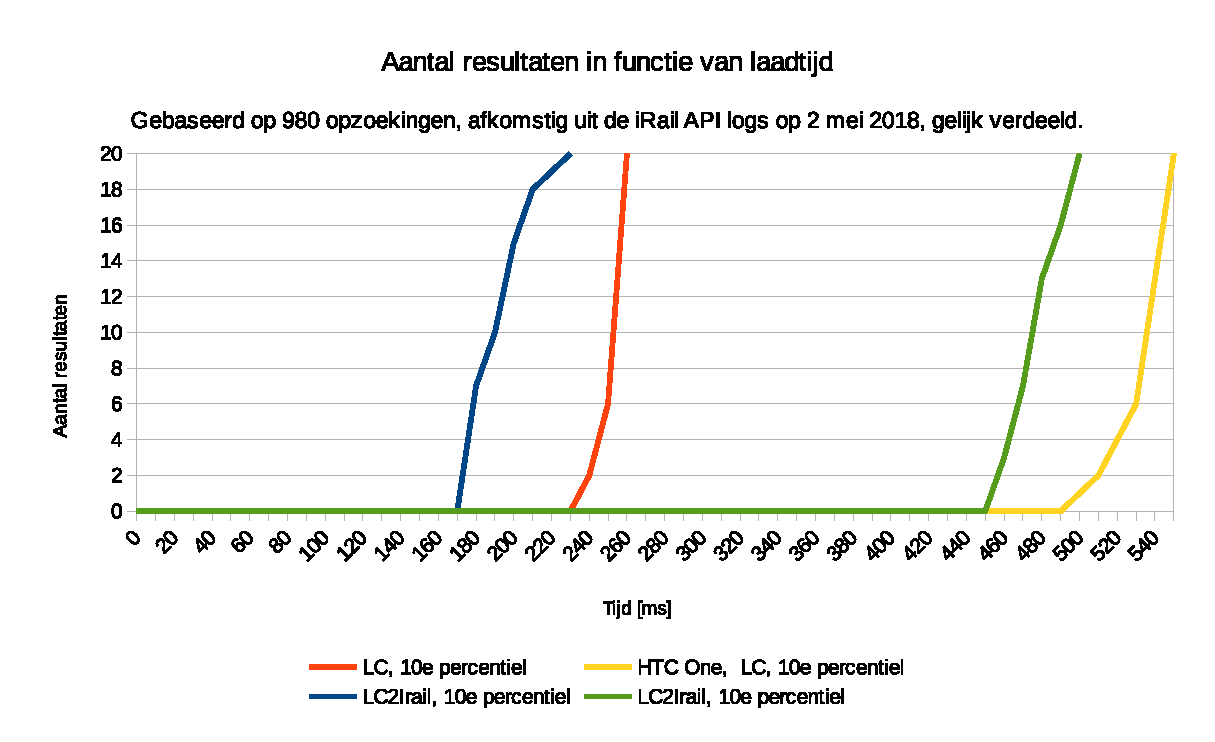
\includegraphics[width=1.00\textwidth]{dief_liveboards_best.eps}
	\caption[Aantal resultaten liveboards in functie van de tijd]{Het aantal resultaten in functie van de verlopen tijd.}
	\label{fig:liveboardsDiefBest}
\end{figure}

\begin{figure}[h]
	\centering
	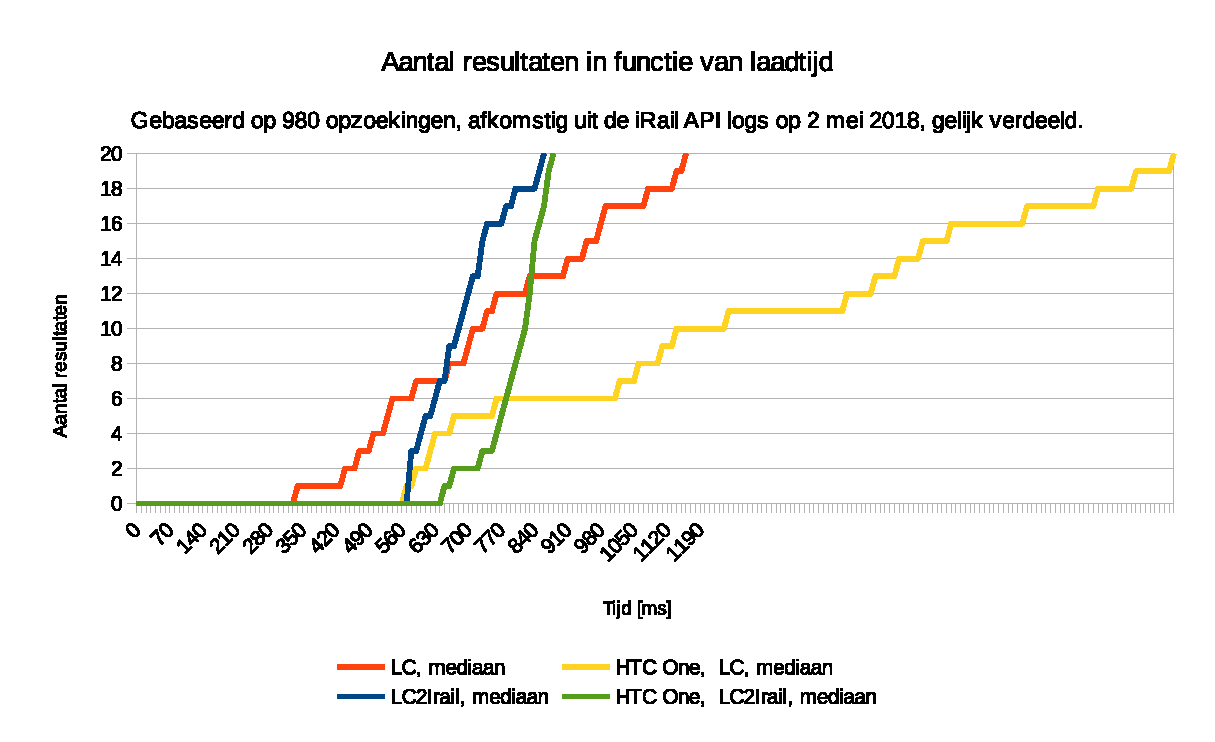
\includegraphics[width=1.00\textwidth]{dief_liveboards_gemiddeld.eps}
	\caption[Aantal resultaten liveboards in functie van de tijd]{Het aantal resultaten in functie van de verlopen tijd.}
	\label{fig:liveboardsDiefAvg}
\end{figure}

\begin{figure}[h]
	\centering
	\includegraphics[width=1.00\textwidth]{dief_liveboards_slechtst.eps}
	\caption[Aantal resultaten liveboards in functie van de tijd]{Het aantal resultaten in functie van de verlopen tijd.}
	\label{fig:liveboardsDiefSlechtst}
\end{figure}

Waneer we nu naar de spreiding van de laadtijden kijken, zichtbaar in figuren \ref{fig:liveboardsBoxplot1} en \ref{fig:liveboardsBoxplot10} zien we ook hier duidelijke verschillen tussen de verschillende methodes. Zo zien we dat bij gebruik van een RPC API de mediaan van de laadtijd ongeveer gelijk is tussen verschillende toestellen, en de interkwartielafstand relatief klein is, wat op een kleine spreiding en dus consistente resultaten duidt. Bij gebruik van Linked Connections zien we duidelijke verschillen tussen de mediaan van de laadtijd bij verschillende toestellen. Ook de interkwartielafstand varieert tussen toestellen: zo is een ouder toestel niet enkel trager, maar is ook de spreiding veel groter, en zijn de resultaten dus minder consistent op oudere (tragere) toestellen.

\subsection{Ervaringen}
Wanneer we nu naar de ervaringen van gebruikers gaan kijken, stemmen deze ongeveer overeen met wat we zouden verwachten na het bekijken van voorgaande grafieken. 

Zoals we in figuren \ref{fig:liveboardsBoxplot1} en \ref{fig:liveboardsBoxplot10} konden zien blijkt uit testen dat de performantie van LC2Irail consistenter is. Ook bij de gebruikerservaring zien we dit terugkomen. Wanneer de ervaren snelheid wordt uitgezet in een boxplot per implementatie, zichtbaar in figuur \ref{fig:liveboardsUx}, zien we net als bij de testen dat voor LC2Irail een heel consistente beoordeling wordt gegeven, terwijl deze voor Linked Connections veel meer uitgespreid, én iets lager ligt.

\begin{figure}[h]
	\centering
	\includegraphics[width=0.80\textwidth]{boxplot_liveboards_ux.eps}
	\caption[Ervaren snelheid van liveboards]{De ervaren snelheid op een schaal 1-7 van vertrekken en aankomsten voor LC2Irail en Linked Connections, gebaseerd op 17 user tests.}
	\label{fig:liveboardsUx}
\end{figure}

Hoewel 12 van de 17 testpersonen aangeeft licht tot extreem tevreden te zijn met de laadsnelheid, geven slechts 2 personen aan dat de lijst met vertrekken sneller laadt bij de lokale implementatie van Linked Connections. Nog eens 3 personen geven aan beide implementaties even snel te ervaren.

Wanneer we gaan kijken naar de verschillen tussen de JSON parsers, blijkt dat beide parsers ongeveer even goed presteren in de ogen van de gebruikers. Respectievelijk 5 op 7 en 7 op 10 gebruikers zijn neutraal of tevreden, en bij beide varianten is er telkens een gebruiker neutraal. Deze vergelijking is echter slechts een indicatie, en is door te kleine steekproeven ongeschikt om te veralgemenen naar een grotere populatie.

Wanneer we kijken naar de gemeten prestatieverschillen tussen beide JSON parsers tijdens de usertests, zien we een duidelijk verschil, waarbij het 90e percentiel van de laadtijd onder de LoganSquare parser lager ligt dan de mediane laadtijd van de org.json parser. Dit verschil lijkt echter geen invloed te hebben op de ervaringen van gebruikers, vermoedelijk omdat men beide reeds als performant genoeg ervaart.

Tot slot werden alle testpersonen ook expliciet gevraagd welke implementatie ze als sneller ervaarden. Hierbij waren de antwoorden verdeeld: acht personen kozen de eerste variant, vier personen hadden geen mening, en vijf personen kozen de tweede variant. Hierbij valt op dat bij de eerste lokale implementatie, 

\section{Routes}

\subsection{Metingen}
\begin{figure}[h]
	\centering
	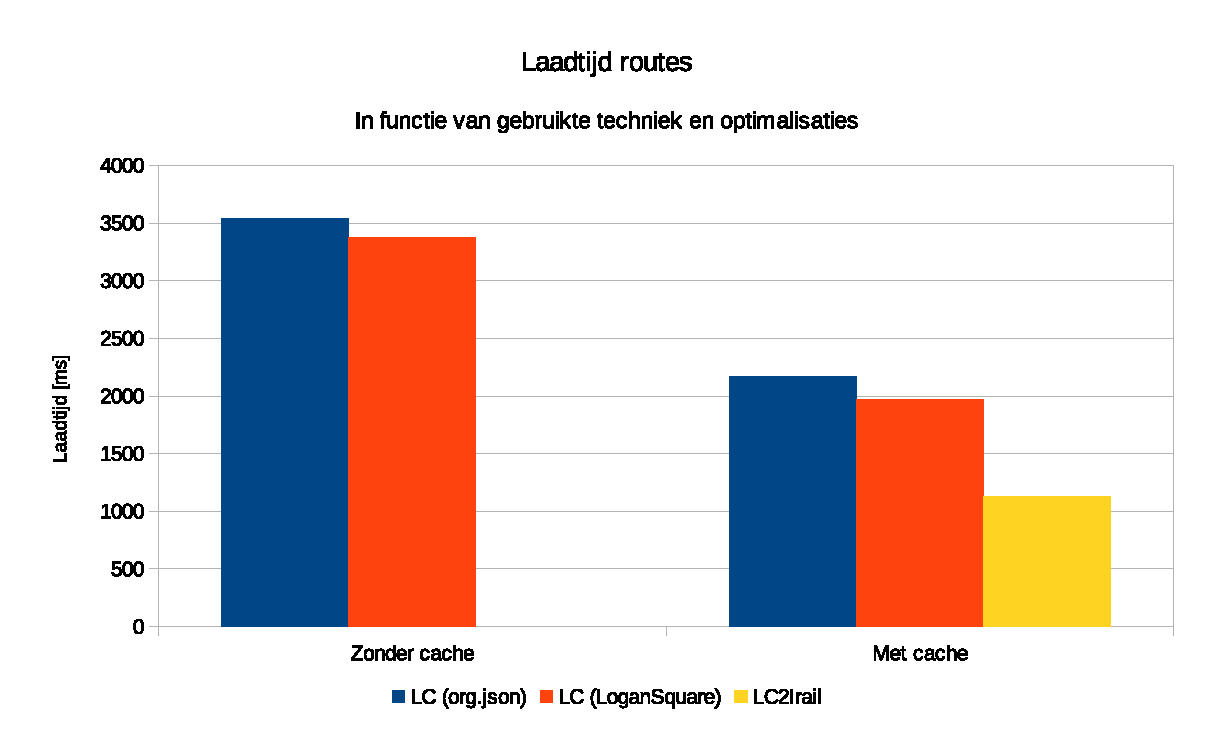
\includegraphics[width=0.80\textwidth]{Optimalisaties_routes.eps}
	\caption[Gemeten laadtijd routes]{De gemeten laadtijd voor routes gebruikmakend van een HTC 10 voor 779 opzoekingen gebaseerd op de iRail logs.}
	\label{fig:routelabtest}
\end{figure}
\begin{table}[h]
	\begin{tabular}{| c | c | c | c | c | c |}
		\hline
		Variant & parser & cache & minimaal (ms) & gemiddelde (ms) & maximaal (ms)\\
		\hline
		LC op toestel & org.json & nee & 401 & 3539 & 8531\\
		LC op toestel & org.json & ja & 221 & 2172 & 6960 \\
		LC op toestel & LoganSquare & nee &  386 & 3374 & 7554 \\
		LC op toestel & LoganSquare & ja  & 233 & 1973 & 7640 \\
		
		LC op server &&&  27 & 1126 & 3374\\
		\hline
	\end{tabular}
	\caption[Gemeten laadtijd routes]{De gemeten laadtijd voor routes gebruikmakend van een HTC 10 voor 779 opzoekingen gebaseerd op de iRail logs.}
	\label{tab:routelabtest}
\end{table}

In tabel \ref{tab:routelabtest} en grafiek \ref{fig:routelabtest} zijn de resultaten zichtbaar van een benchmark waarbij 779 routes opgezocht werden, ongeveer 5\% van de opzoekingen door gebruikers op 2 mei 2018. Telkens is de minimale, gemiddelde en maximale responstijd gemeten. Dit zowel gebruikmakend van de standaard JSON parser (\foreign{org.json}) en gebruikmakend van de \foreign{LoganSquare} parser. Ook werd de test herhaald met cache in- en uitgeschakeld, om zo het effect hiervan te meten. Tot slot werd dezelfde test herhaald gebruikmakend van data afkomstig van de LC2Irail web applicatie om een vergelijking tussen de twee methodes te kunnen maken. Deze cijfers geven slechts een indicatie van de snelheid - een volledige en diepgaande statistische analyse van de performantieverschillen tussen verschillende implementatiedetails van dezelfde techniek valt wegens tijdsgebrek buiten het bereik van deze masterproef.

Net zoals bij liveboards is ook hier de invloed van de cache duidelijk merkbaar. Vergeleken met dezelfde analyse voor Liveboards (figuur \ref{fig:liveboardlabtest}), zien we hier een minder groot verschil tussen de parsers: er moeten grote hoeveelheden data verwerkt worden, en het algoritme om de data te verwerken is het zwaarst van de drie endpoints.

Om ook hier een exact beeld te vormen van de prestaties, maken we ook hier een duizendtal opzoekingen. Hiervoor kiezen we telkens de vijfde opzoeking uit de iRail logs. Voor elke route wordt gepoogd 10 resultaten geladen. De resultaten hiervan zijn zichtbaar in grafieken \ref{fig:routesDiefBest}, \ref{fig:routesDiefAvg} en \ref{fig:routesDiefSlechtst}, respectievelijk voor het tiende, vijftigste en negentigste percentiel.

\begin{figure}[h]
	\centering
	\includegraphics[width=1.00\textwidth]{dief_routes_best.eps}
	\caption[Aantal resultaten routes in functie van de tijd]{Het aantal resultaten in functie van de verlopen tijd.}
	\label{fig:routesDiefBest}
\end{figure}

\begin{figure}[h]
	\centering
	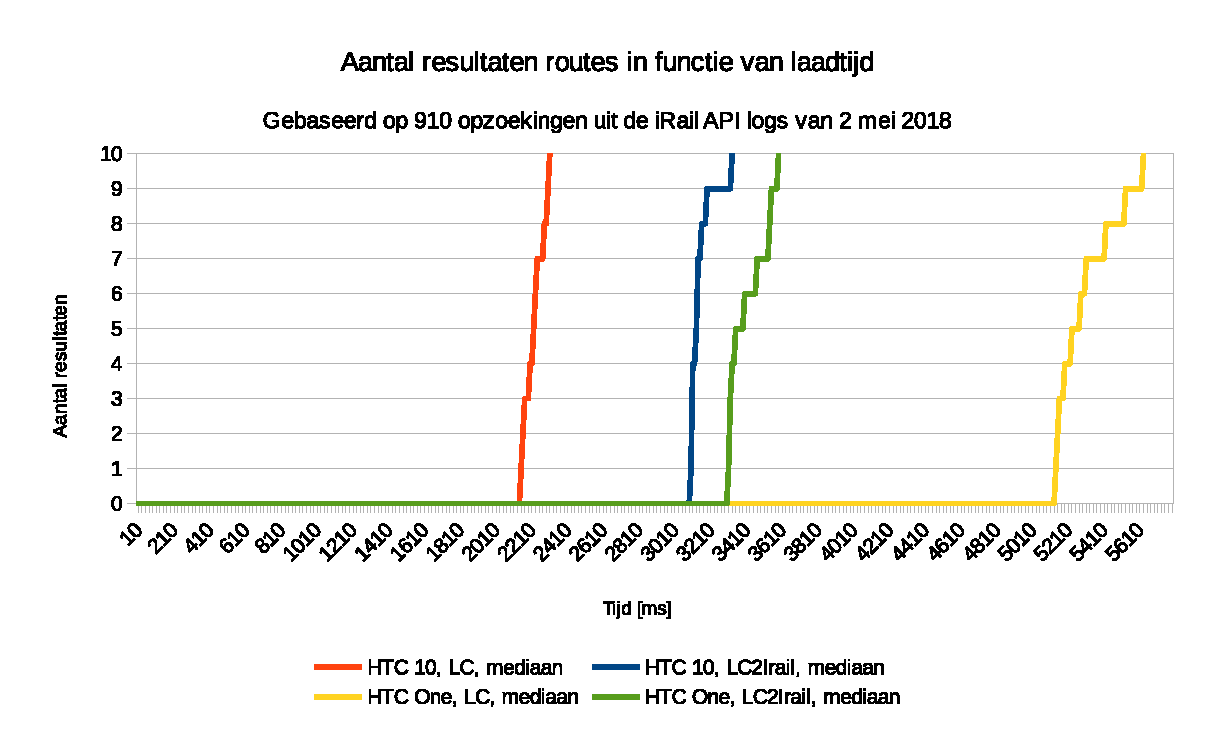
\includegraphics[width=1.00\textwidth]{dief_routes_gemiddeld.eps}
	\caption[Aantal resultaten routes in functie van de tijd]{Het aantal resultaten in functie van de verlopen tijd.}
	\label{fig:routesDiefAvg}
\end{figure}

\begin{figure}[h]
	\centering
	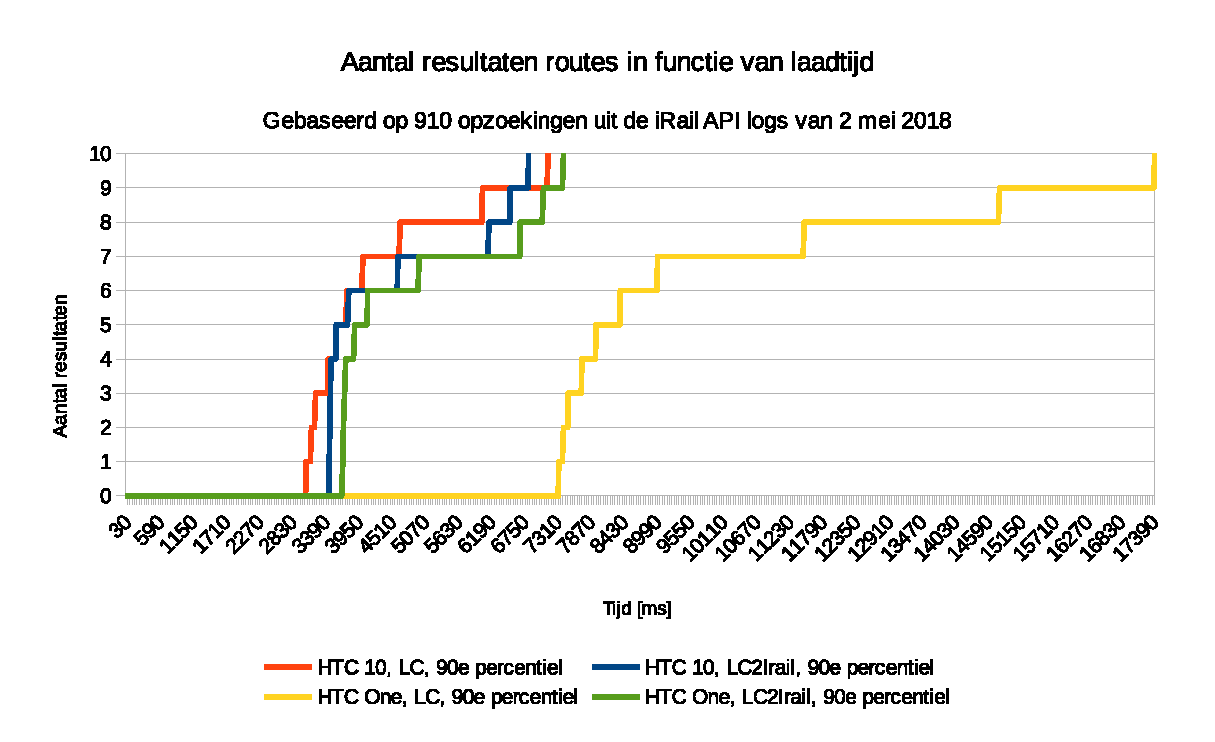
\includegraphics[width=1.00\textwidth]{dief_routes_slechtst.eps}
	\caption[Aantal resultaten routes in functie van de tijd]{Het aantal resultaten in functie van de verlopen tijd.}
	\label{fig:routesDiefSlechtst}
\end{figure}

Uit deze grafieken kunnen we opnieuw duidelijke verschillen zien:
\begin{itemize}
	\item In alle grafieken en voor alle testen, hebben de curves een gelijkaardige vorm, waarbij er na een relatief lange wachttijd aan snel tempo resultaten geladen worden: in het geval van Linked Connections is voor de eerste opzoeking telkens een relatief grote hoeveelheid data nodig is, waarna slechts één of twee extra pagina's moeten opgehaald worden om het volgend resultaat te bepalen. In het geval van LC2Irail worden resultaten in grote blokken binnengehaald, waarbij vanaf de tweede opzoeking reeds veel data in cache zit. In het geval van LC2Irail worden resultaten ook onmiddelijk voor grote intervals opgehaald, om zo het aantal verzoeken te beperken. 
	\item Terwijl in het alle gevallen Linked Connections beter presteert op de HTC 10, presteert het slechter op de HTC One. 
	\item Opnieuw presteert LC2Irail op beide toestellen gelijkaardig, met slechts een kleine verschuiving in tijd tussen beide curves.
	\item Terwijl in het slechtste geval bijna alle varianten gelijk presteren, loopt Linked Connections op de HTC 10 enorm achter.
\end{itemize}

Wanneer we nu specifiek naar de verdelingen kijken, gevisualiseerd door middel van box plots in figuur \ref{fig:routesBoxplot1} en \ref{fig:routesBoxplot10}, Zien we ook hier duidelijk hoe LC2Irail gelijke prestaties heeft op beide toestellen, terwijl de prestaties van Linked Connections sterk variëren per toestel. Op de HTC 10 zal al meer dan 75\% van de opzoekingen geladen zijn op het moment dat LC2Irail op hetzelfde toestel minder dan 25\% van de verzoeken beantwoordt heeft. Op het HTC One toestel is dit echter omgekeerd, en nog extremer. 

\begin{figure}[h]
	\centering
	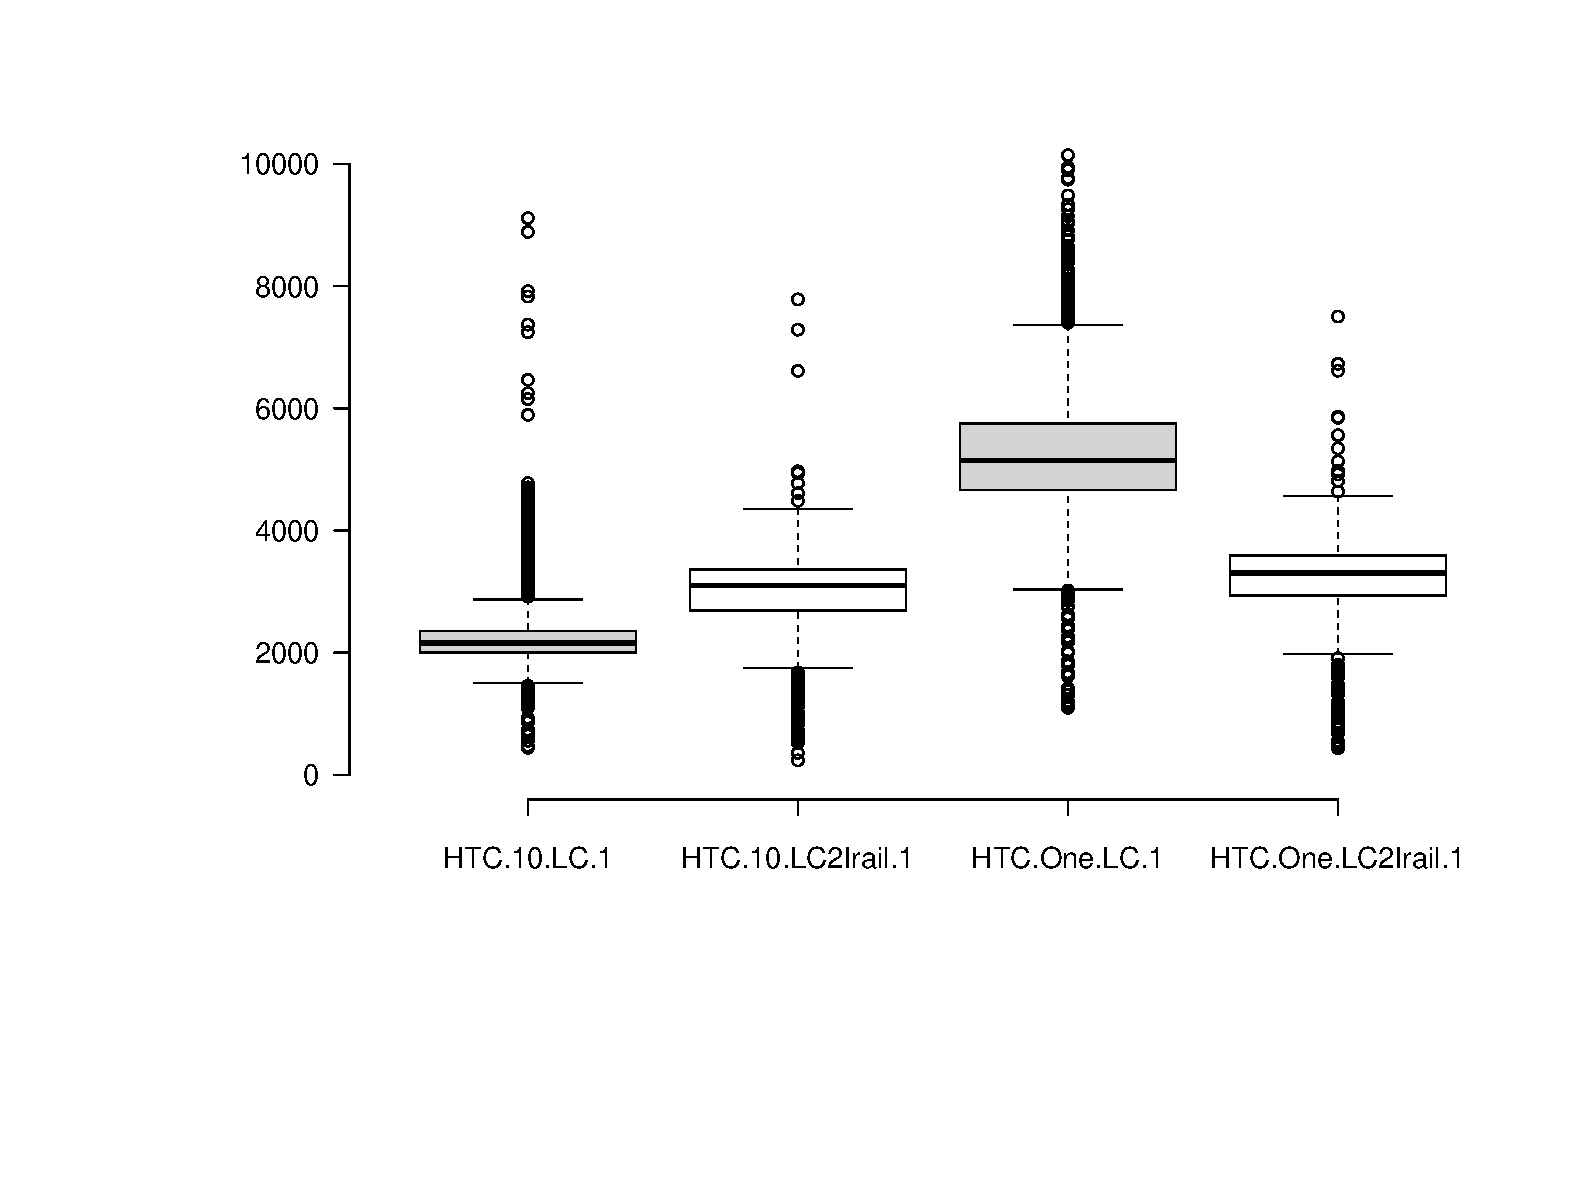
\includegraphics[width=0.80\textwidth]{boxplot_routes_1.eps}
	\caption[Laadtijd eerste resultaat route in functie van toestel en technologie]{Laadtijd eerste resultaat route in functie van toestel en technologie.}
	\label{fig:routesBoxplot1}
\end{figure}

\begin{figure}[h]
	\centering
	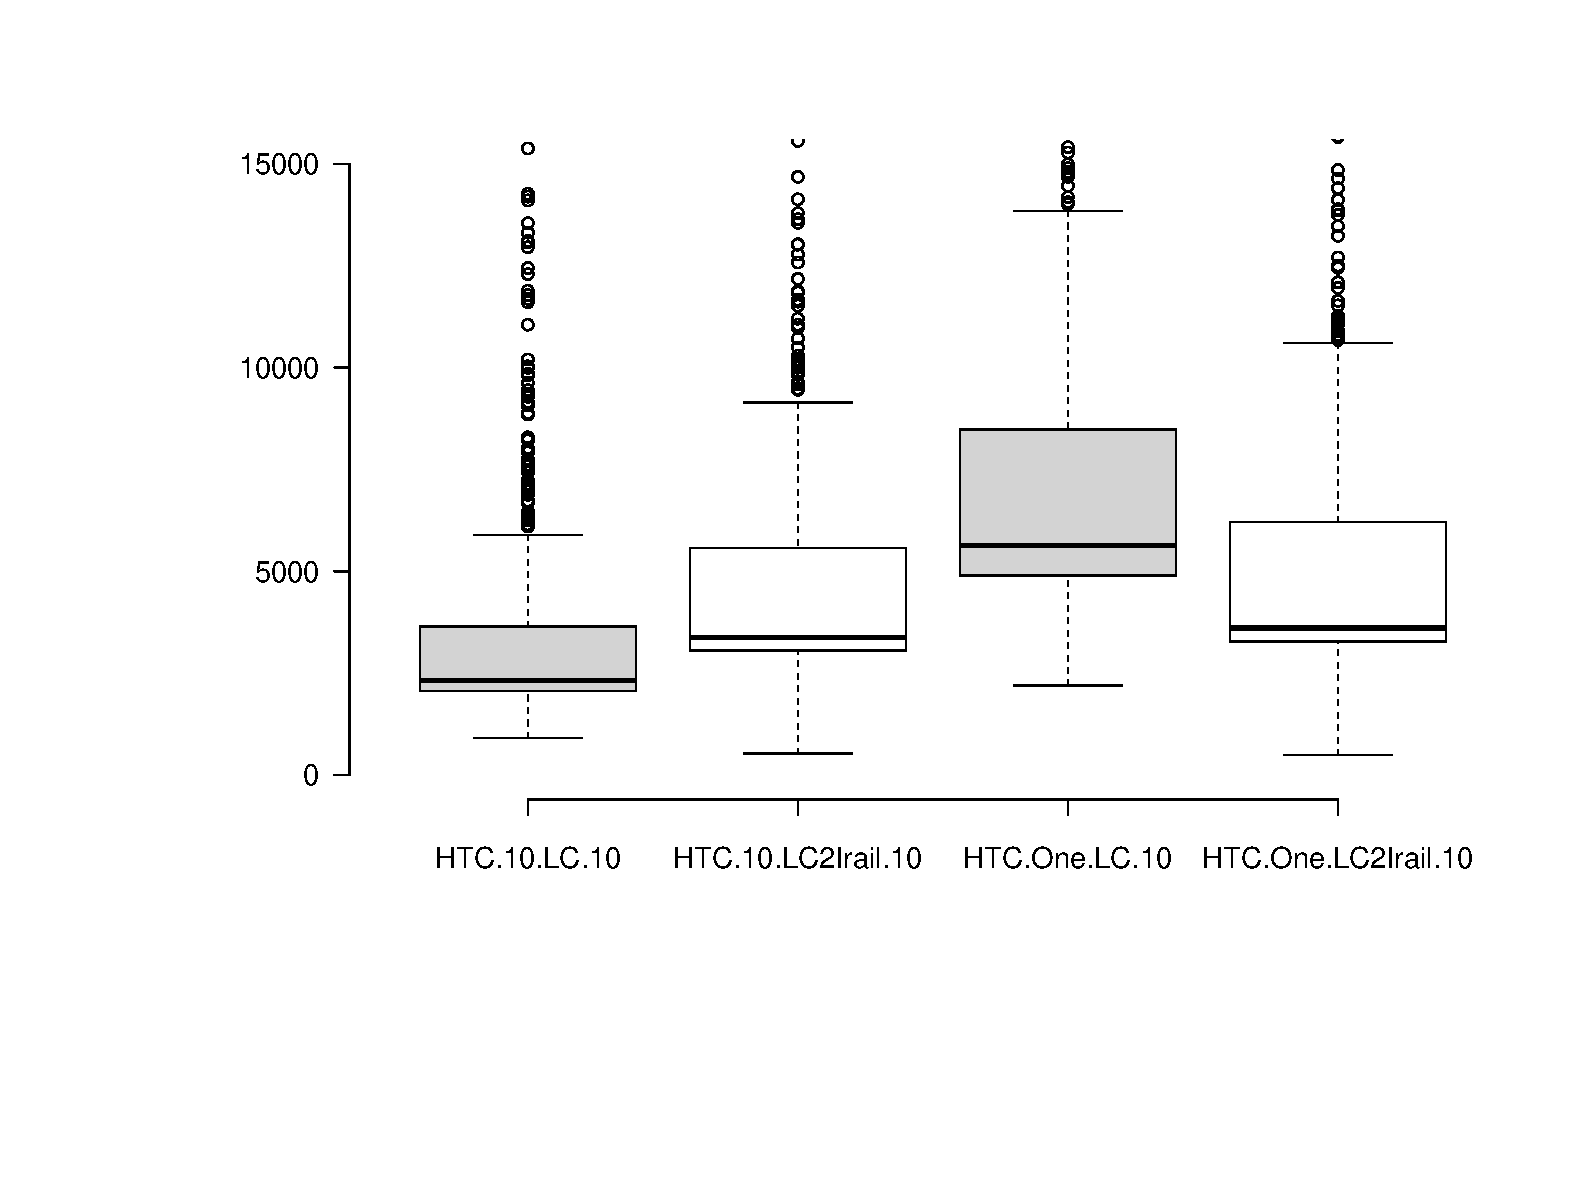
\includegraphics[width=0.80\textwidth]{boxplot_routes_10.eps}
	\caption[Laadtijd tiende resultaat route in functie van toestel en technologie]{Laadtijd tiende resultaat route in functie van toestel en technologie.}
	\label{fig:routesBoxplot10}
\end{figure}

\subsection{Ervaringen}

Op vlak van gebruikerservaring verwachten we dat gebruikers net zoals bij Liveboards de implementatie op basis van LC2Irail consistenter zullen beoordelen, en dat snelheid voor beide implementaties ongeveer gelijk ervaren wordt.

Wanneer we nu de resultaten van user testing vergelijken met de verwachtingen, blijken deze verwachtingen grotendeels in vervulling te gaan. In figuur \ref{fig:routesUx} is te zien dat de prestaties van LC2Irail iets consistenter beoordeeld worden, en LC2Irail tevens een betere beoordeling krijgt dan Linked Connections. 

Wanneer we voor routes beide JSON parsers vergelijken, zien we dat voor de LoganSquare parser de proefpersonen een meer uitgesproken mening hadden: er waren zowel meer tevreden als ontevreden personen, terwijl bij de \foreign{org.json} parser veel mensen neutraal waren. Dit gaat echter in tegen een praktijktest waarbij enkele gebruikers achtereenvolgens een versie gebruikmakend van de \foreign{org.json} en \foreign{LoganSquare} parser voorgeschoteld kregen, gaven deze telkens aan de versie op basis van \foreign{LoganSquare} sneller te ervaren, zowel op goedkope als dure smartphones. Hieruit besluiten we dat de gebruikerstests, opgedeeld per parser, te kleine steekproeven zijn om een algemene conclusie te vormen over de invloed van de parsers.

\begin{figure}[h]
	\centering
	\includegraphics[width=0.80\textwidth]{boxplot_routes_ux.eps}
	\caption[Ervaren snelheid van routes]{De ervaren snelheid op een schaal 1-7 van routes voor LC2Irail en Linked Connections, gebaseerd op 17 user tests.}
	\label{fig:routesUx}
\end{figure}

\section{Voertuigen}

\subsection{Metingen}
Het opzoeken van het traject dat een voertuig aflegt heeft als groot verschil dat incrementele resultaten niet door de gebruikte applicatie ondersteund worden. De reden hiervoor is dat het traject van het voertuig het enige en volledige resultaat is dat de gebruiker wenst, in tegenstelling tot liveboards en routes, waar de gebruiker niet het volledige, maar slechts een deel van het resultaat wenst te zien. 

Dit is ook de opzoeking die het meeste data vereist bij Linked Connections: alle pagina's moeten doorzocht worden op connecties met betrekking tot één specifiek voertuig. Dit voertuig komt slechts in een relatief beperkt aantal pagina's voor, gezien het voertuig slechts enkele uren rijdt, en het tijdstip van eerste vertrek en aankomst onbekend zijn. Zoals eerder vermeld %TODO: referntie
zijn hier enkele oplossingen voor, zoals het gebruik van een index. We definiëren een index in deze context als een lijst van alle treinen voor een bepaalde periode (in dit geval mei 2018) en het tijdstip van hun eerste vertrek.

Om een idee te krijgen van de invloed van deze index, alsook van het gebruik van een cachegeheugen voor de Linked Connections pagina's bij deze opzoekingen, werden 102 voertuigen opgezocht, voor alle combinaties van cache en index gebruik. Tevens werd een extra test gedaan met een cache die in het RAM geheugen geplaatst wordt (in tegenstelling tot het flashgeheugen van het toestel), en een vergelijkende test waarbij de Linked Connections server gebruikt werd. De minimale, gemiddelde en maximale opzoektijd hiervoor is te zien in tabel \ref{tab:vehiclelabtest}. De gemiddelde resultaten zijn tevens gevisualiseerd in figuur \ref{fig:vehiclelabtest}.

\begin{figure}[ht]
	\centering
	\includegraphics[width=1.00\textwidth]{Optimalisaties_voertuigen.eps}
	\caption[Gemeten laadtijd voertuigen]{De gemeten laadtijd voor voertuigen gebruikmakend van een HTC 10 voor 102 opzoekingen gebaseerd op de iRail logs. }
	\label{fig:vehiclelabtest}
\end{figure}

\begin{table}[ht]
	\begin{tabular}{| c | c | c | c | c | c | c |}
		\hline
		Variant & parser & cache & index & minimaal (ms) & gemiddelde (ms) & maximaal (ms)\\
		\hline
		LC op toestel & org.json & nee & nee & 540 & 6764 & 12676 \\
		LC op toestel & org.json & ja & nee & 483 & 6488 & 10921 \\
		
		LC op toestel & org.json & nee & ja & 2638 & 4443 & 10956 \\
		LC op toestel & org.json & ja & ja &  2440 & 4066 & 6003\\
		LC op toestel & org.json & RAM & ja & 2263 & 3912 & 5763 \\
		LC op toestel & LoganSquare & nee & ja &  1860 & 3283 & 5374 \\
		LC op toestel & LoganSquare & ja  & ja & 1195 & 1925 & 2888 \\
		
		LC op server &&&&  264 & 713 & 5068 \\
		\hline
	\end{tabular}
	\caption[Gemeten laadtijd voertuigen]{De gemeten laadtijd voor voertuigen gebruikmakend van een HTC 10 voor 102 opzoekingen gebaseerd op de iRail logs. }
	\label{tab:vehiclelabtest}
\end{table}

Het is duidelijk dat de standaard implementatie zeer slecht presteert. Ook het gebruik van een cachegeheugen brengt hierbij niet veel beterschap. Wanneer echter een index toegevoegd worden, is een drastische verbetering merkbaar. Het gemiddelde daalt in deze beeperkte test met ongeveer een derde. Toevoeging van een cachegeheugen, op flash of in het RAM geheugen, brengt ook hier slechts weinig beterschap. 

Een tweede grote verbetering kan behaald worden door het gebruik van de eerder besproken LoganSquare parser. Hierbij zien we ook een veel grotere verbetering door cachegebruik dan bij de org.json parser. Dit is logisch, gezien bij het gebruik van de LoganSquare parser het verwerken van de data relatief gezien minder tijd in beslag neemt - het ophalen van data wordt dus belangrijker. Op het eerste zicht blijven alle lokale varianten veel trager dan de serverimplementatie, die sneller door pagina's kan zoeken.

We onderzoeken nu het verschil tussen de lokale implementatie en de serverimplementatie in detail. Hiervoor zoeken we 1620 voertuigen op die plaatsvinden op 6 mei 2018. Dit wordt enerzijds gedaan voor de lokale implementatie die gebruik maakt van de LoganSquare parser, cache en lokale index, en anderzijds voor de serverimplementatie, die server-side over dezelfde index en een cache beschikt.

Wanneer we kijken naar de box-plot van de responstijd, weergegeven in figuur \ref{fig:vehicleboxplot}, zien we dat de lokale implementatie duidelijk slechter presteert. Op beide toestellen is LC2Irail sneller dan Linked Connections. Bij de HTC 10, een snel toestel, valt dit nog enigszins mee, maar op de HTC One zijn de meeste resultaten binnen 3000 milliseconden geladen, terwijl op dat moment nog geen 25\% van de opzoekingen via Linked Connections uitgevoerd werd. Ook zien we hier dat LC2Irail consistente prestaties biedt: beide box plots zijn praktisch identiek, op wat uitlopers na. Voor Linked Connections zien we echter dat, net zoals voor het opzoeken van liveboards en routes, de spreiding van de benodigde tijd afhangt van het toestel: een traag toestel heeft een grotere variatie in de laadtijd.

\begin{figure}[h]
	\centering
	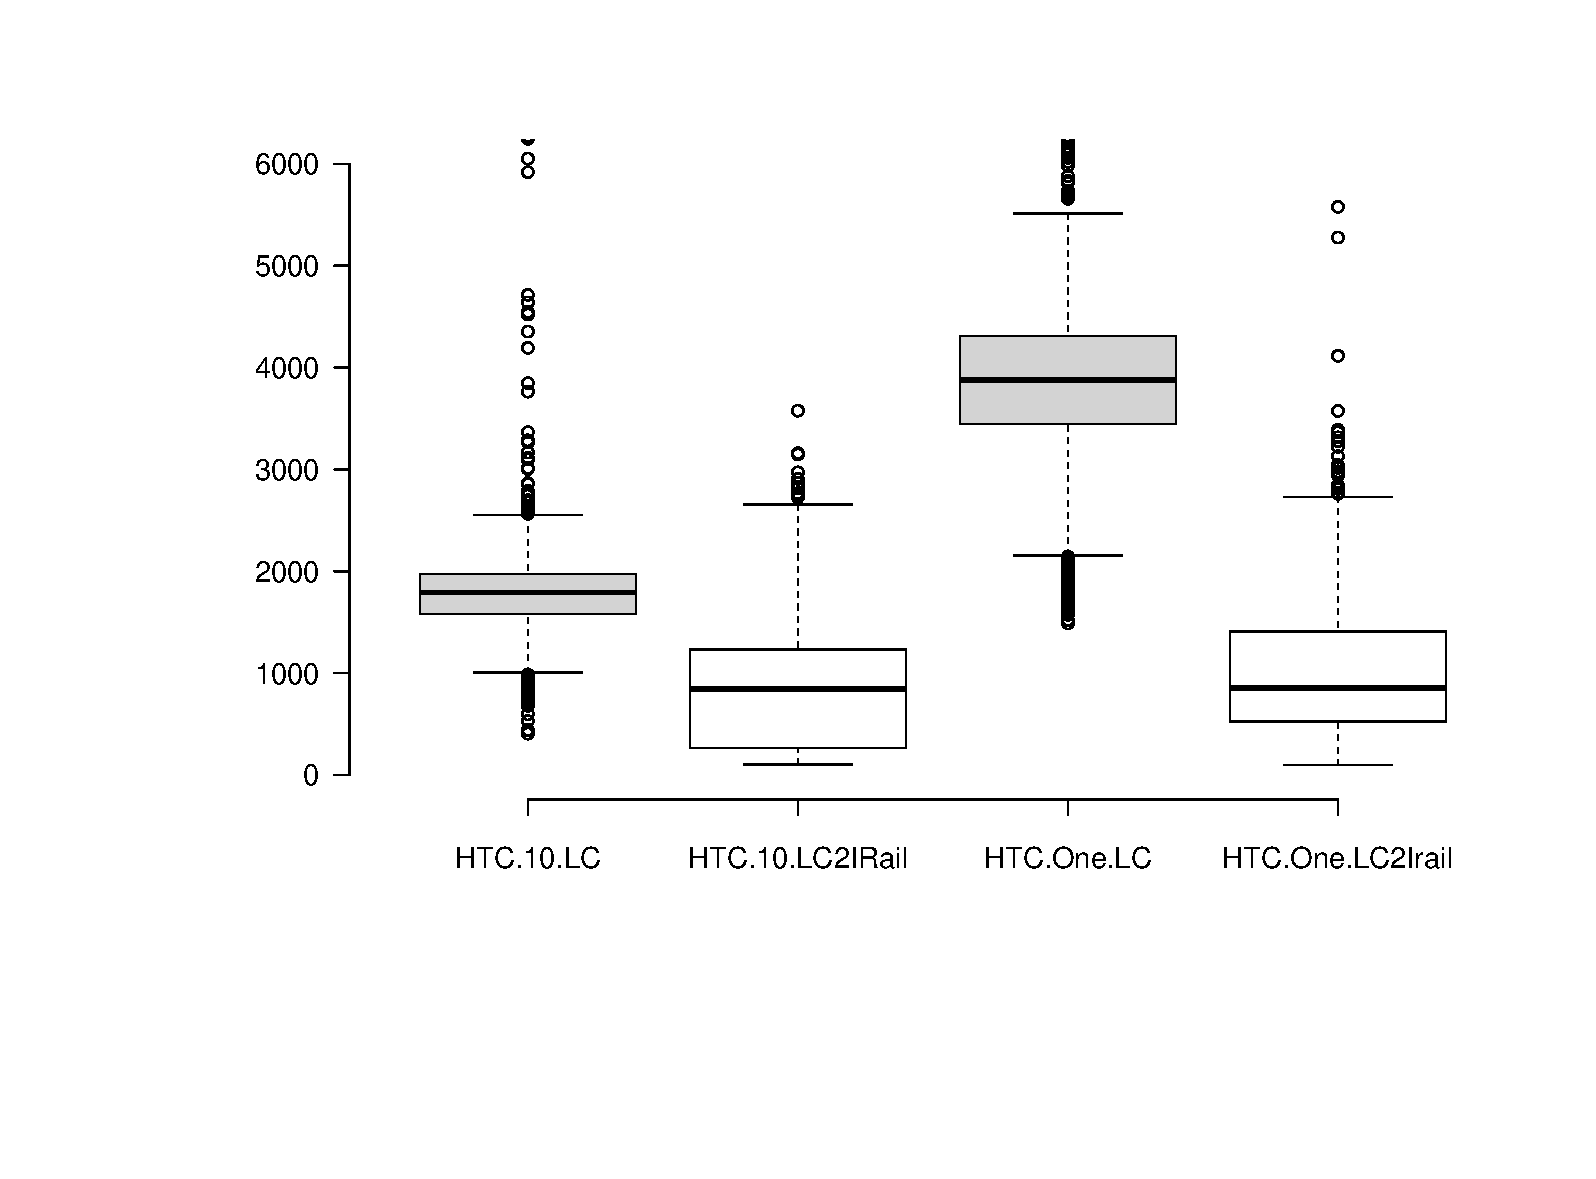
\includegraphics[width=1.00\textwidth]{boxplot_vehicles.eps}
	\caption[Prestaties voor het laden van voertuigen]{De prestaties voor het laden van voertuigen, gemeten door alle voertuigen, beschreven in Linked Connections, voor 6 mei op te zoeken.}
	\label{fig:vehicleboxplot}
\end{figure}

%\begin{figure}[h]
%	\centering
%	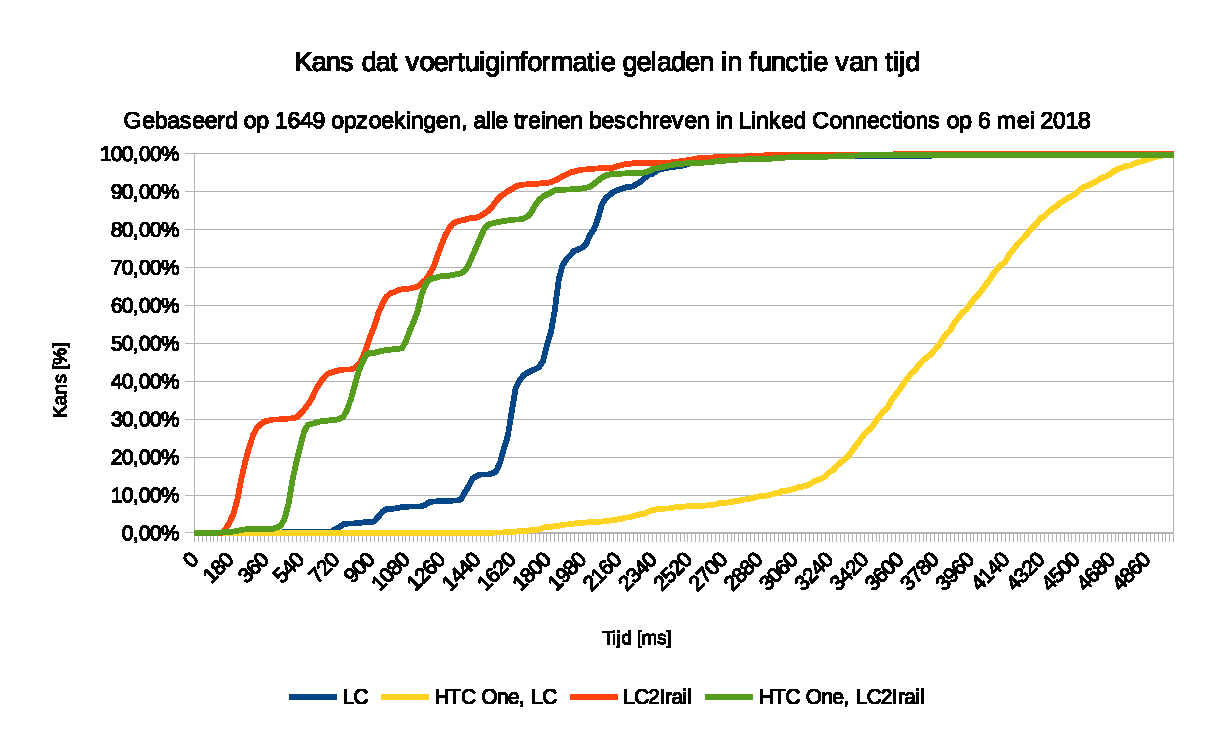
\includegraphics[width=1.00\textwidth]{distribution_vehicle_loading_cummulatief.eps}
%	\caption[Cummulatieve kans op laden van voertuig]{De kans dat een voertuig geladen is in functie van de verlopen tijd.}
%	\label{fig:vehiclecummulatief}
%\end{figure}

\subsection{Ervaringen}
Wanneer we nu de resultaten van de user-testing bekijken, zien we zoals verwacht dat het laden van voertuigen beduidend slechter scoort wanneer de lokale Linked Connections implementatie gebruikt wordt, vergeleken met wanneer de serverimplementatie gebruikt werd. In figuur \ref{fig:vehicleboxplot} is dit duidelijk zichtbaar. Zo beoordelen de meeste gebruikers Linked connections slechts als "gemiddeld", terwijl de meerderheid van de gebruikers de LC2Irail variant als "Zeer snel" bestempelde. Ook zien we hier, net als bij liveboards en routes, dat er voor Linked Connections een veel grotere spreiding is in de gegeven antwoorden, terwijl  bij LC2Irail iedereen het er over eens lijkt dat deze implementatie snel is.

\begin{figure}[h]
	\centering
	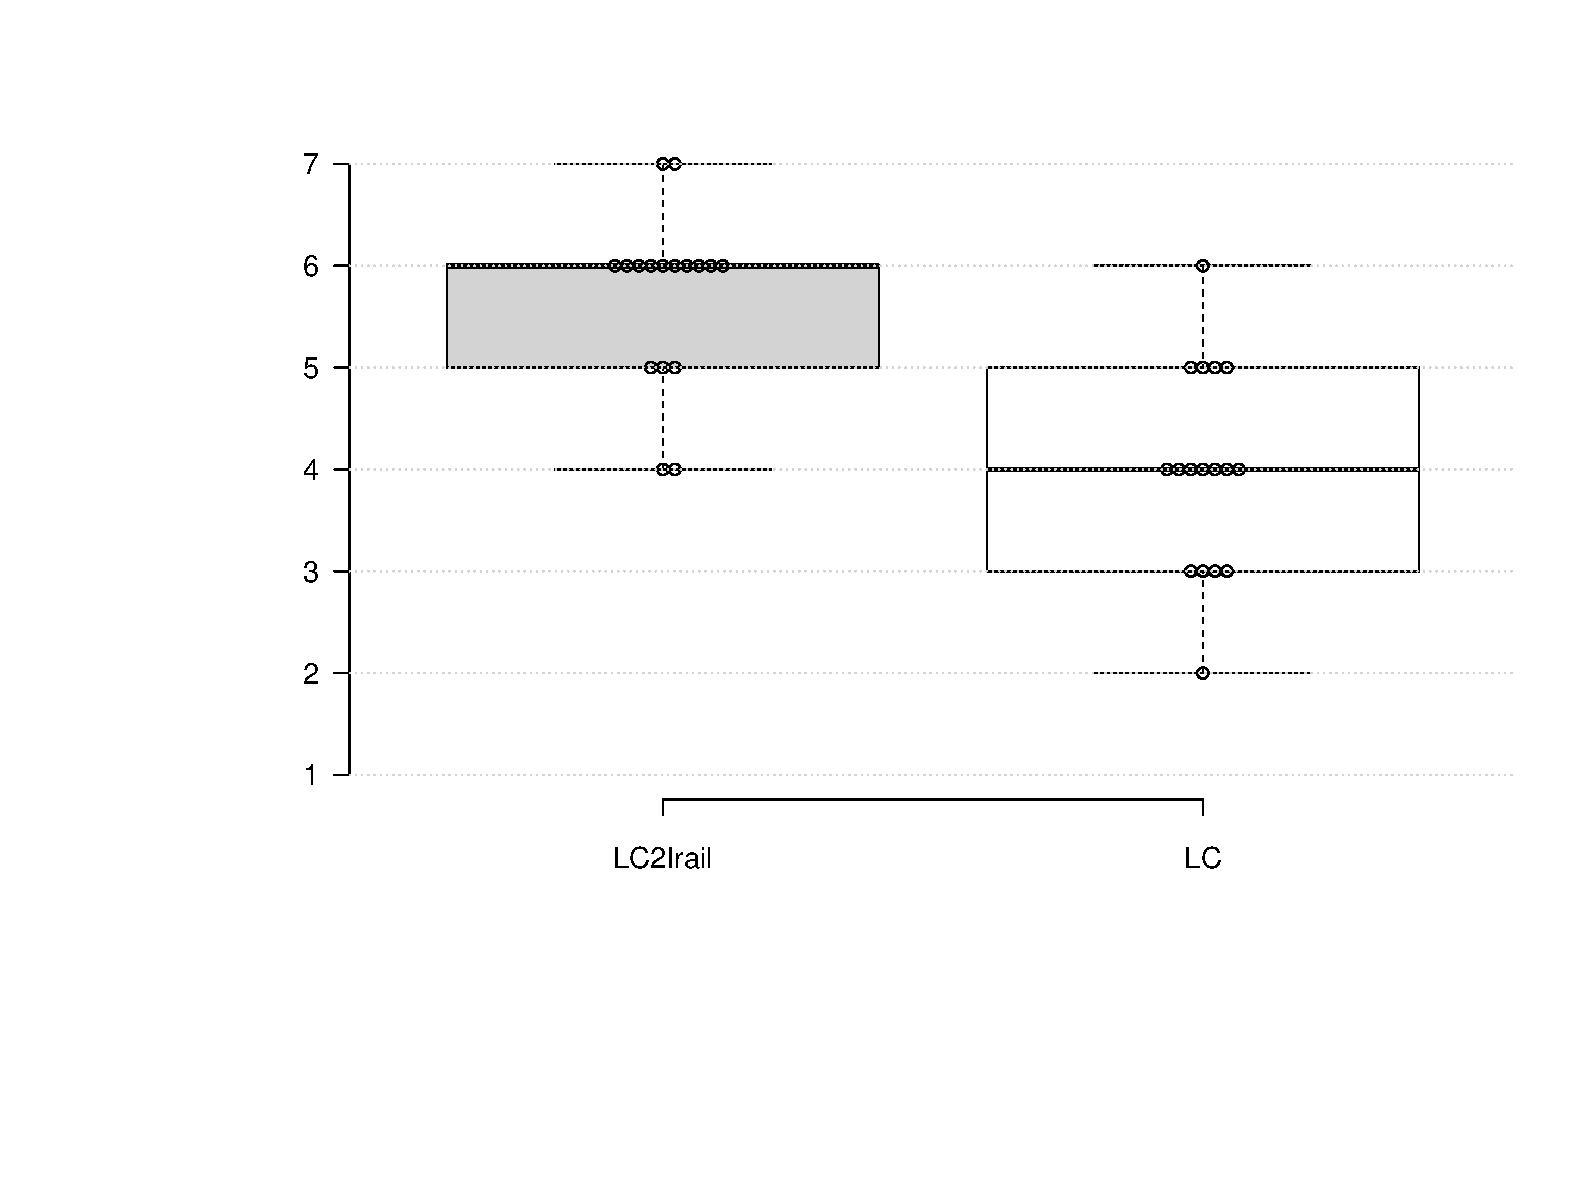
\includegraphics[width=1.00\textwidth]{boxplot_vehicles_ux.eps}
	\caption[Ervaren snelheid van routes]{De ervaren snelheid op een schaal 1-7 van routes voor LC2Irail en Linked Connections, gebaseerd op 17 user tests.}
	\label{fig:vehiclesUx}
\end{figure}

Personen die de lokale implementatie op basis van LoganSquare testten, beoordeelden de laadtijd iets beter vergeleken met de groep die de implementatie op basis van de \foreign{org.json} parser testte. Ondanks dat de testgroep onvoldoende groot was om een veralgemening te kunnen maken, kunnen we wel stellen dat er een grote kans is dat verbeteringen in de implementatie de snelheid verder omlaag kunnen brengen, en zo de gebruikerservaring kunnen verbeteren. Gezien bij het berekenen van voertuigen het meeste data nodig is, is hier de impact van implementatiedetails het grootst.


Wanneer de gebruiker gevraagd werd te kiezen, koos slechts één gebruiker voor de lokale implementatie in dit onderdeel. Vijf gebruikers hadden geen specifieke voorkeur voor een specifieke implementatie, ook al beoordeelden vier van hen de lokale implementatie als trager.
Hieruit concluderen we dat gebruikers de laadtijd van voertuigdata acceptabel vinden wanneer deze onder 1 seconde blijft. Een seconde langer laden, wat het geval is bij de lokale implementatie, wordt door de meeste personen niet meer als snel ervaren.


\section{Keuze van de gebruiker}

Voor alle soorten informatie (liveboards, routes, en voertuigen) lijkt Linked Connections een slechtere gebruikerservaring dan LC2Irail, in termen van laadtijd. Hierbij dienen we op te merken dat dit verschil bij liveboards slechts zeer beperkt is, en het laden nog steeds als snel werd ervaren. Voor routes bestempelden enkele personen Linked Connections als traag, maar blijft het verschil beperkt. Bij voertuigen blijkt echter dat Linked Connections door drie kwart van de gebruikers als trager werd ervaren, waarbij Linked Connections niet enkel relatief slechter scoort, maar ook in absolute termen slechts door een minderheid van de gebruikers als snel wordt ervaren. 

Dit zien we ook terug in de antwoorden wanneer gebruikers gevraagd werd te kiezen tussen beide implementaties. Voor vertrekken zijn er vier gebruikers die beide implementaties even snel vinden, terwijl van de overige 13 slechts vijf kiezen voor Linked Connections. Bij routes en voertuigen scoort Linked Connections zoals verwacht slechter: er zijn respectievelijk slechts twee en een gebruiker die voor Linked Connections kiezen zijn. Hierbij zijn er respectievelijk twee en vijf gebruikers die geen verschil tussen de implementaties merkten.

Terwijl de meerderheid van de gebruikers steeds voor LC2Irail koos, kantelt deze balans echter volledig om wanneer gebruikers worden gevraagd om met alle aspecten rekening te houden: zodra ook  offline gebruik meespeelt, kiezen nog maar vijf gebruikers voor LC2Irail. Twee gebruikers zijn onbeslist, de andere tien gebruikers kiezen voor Linked Connections. Hieruit blijkt duidelijk dat gebruikers enige snelheid willen opgeven in ruil voor offline opzoekingen. Zeven gebruikers laten weten dat ze een hybride systeem ideaal zou zijn, waarbij de snelheid van LC2Irail gecombineerd wordt met Linked Connections als offline alternatief. Wanneer deze gebruikers alsnog verplicht werden te kiezen, waren hun keuzes gelijk verdeeld, afhankelijk van de persoonlijke nood om offline te kunnen opzoeken.

\section{Beperkingen}
\subsection{Kleine steekproef voor user testing}
Zoals eerder vermeld ontbreekt op het moment van schrijven nog cruciale informatie in Linked Connections, zoals of een voertuig al dan niet afgeschaft is, en op welk perron een voertuig aankomt. Hierdoor moesten we terugvallen op user-testing onder begeleiding, om gebruikers aan te sporen hun gebruikelijke opzoekingen te doen en te polsen naar hun ervaringen. Dit neemt relatief veel tijd in beslag, waardoor weinig mensen én zin, én tijd hebben. Voorts neemt deze methode van testen ook veel tijd in beslag voor de onderzoeker. 

De groep testgebruikers is wel gevarieerd, zowel in persoonlijke eigenschappen zoals leeftijd, als in reisgewoontes per trein. Wanneer de gehele testgroep duidelijk de voorkeur geeft aan een bepaalde variant, kunnen we deze keuze veralgemenen naar de gehele populatie. Wanneer er echter geen grote meerderheid voor eenzelfde variant kiest, moeten we voorzichtig zijn met conclusies.

\subsection{Beperkt aantal unieke toestellen getest}
Uit de voorgaande secties blijkt dat het gebruikte toestel van groot belang is voor de prestaties van de lokale Linked Connections implementatie. Tijdens het user-testen werd gebruik gemaakt van twaalf verschillende smartphones. Dit aantal is relatief beperkt in vergelijking met het aanbod op de huidige smartphonemarkt. Eventuele verder onderzoek zal de prestaties van Linked Connections op verschillende toestellen moeten vastleggen.

\subsection{Processorverbruik niet meetbaar}
De Android CPU Profiler beïnvloed de prestaties van de applicatie zodanig dat het onmogelijk is om een correct beeld te krijgen van het processorverbruik. Er kan een beeld gevormd worden welke onderdelen van de applicatie het meest processortijd vragen, maar exacte tijdsmetingen zijn niet mogelijk. Deze problemen worden ook door andere Android ontwikkelaars op internet beschreven\footnote{\url{https://stackoverflow.com/questions/49555983/background-concurrent-copying-gc-freed}}. Deze problemen treden op door de nieuwe Android CPU profiler, die zelf teveel processortijd op het apparaat vereist.

\subsection{Prestaties zijn sterk afhankelijk van implementatiedetails}
Zoals blijkt uit grafieken %TODO: REFERENTIE
is de performantie van de lokale Linked Connections implementatie sterk afhankelijk van details in de implementatie - Het is dus niet enkel belangrijk om de algoritmes te optimalizeren, maar ook om rekening te houden met processen zoals Garbage Collection. Dit werd pas in een gevorderd stadium van de proef vastgesteld. Het is mogelijk dat de resultaten in dit onderzoek nog verder verbeterd kunnen worden door dezelfde algoritmes efficiënter te implementeren.
% !TeX spellcheck = nl_NL
\begin{savequote}[0.55\linewidth]
	``It’s difficult to imagine the power that you’re going to have when so many different sorts of data are available.''
	\qauthor{\textasciitilde Tim Berners-Lee}
\end{savequote}

\chapter{Conclusie}
\label{chap:interpretatie}

We zullen nu de resultaten, besproken in hoofdstuk~\ref{chap:resultaten}, interpreteren om zo een antwoord te vinden op de in sectie~\ref{sec:onderzoeksvraag} geuite vragen.

\paragraph{Onderzoeksvraag}  \textbf{Verbetert de user experience en user perceived perforance van een applicatie voor openbaar vervoer wanneer gebruik gemaakt wordt van Linked Connections in plaats van traditionele RPC API's?}\\

Voor liveboards blijkt dat afhankelijk van het gebruikte toestel Linked Connections concurrentieel is op vlak van snelheid, zowel gemeten als ervaren. Dit wordt ook duidelijk gereflecteerd in de ervaren snelheid, die door een groot deel van de gebruikers als `redelijk snel' of beter aangeduid wordt. Toch blijkt dat de ervaren snelheid iets onderdoet voor die van een RPC API.

Bij routes en voertuigen wordt de achterstand van Linked Connections tegenover RPC steeds groter. Gebruikers zijn het ook absoluut niet met elkaar eens over de ervaren snelheid, terwijl voor LC2Irail vrijwel alle gebruikers voor (ongeveer) dezelfde snelheid ervoeren.

Hieruit trekken we de conclusie dat Linked Connections enorm afhankelijk is van het gebruikte toestel,  waarbij toestellen met meer processorkracht en/of werkgeheugen een duidelijk voordeel hebben ten opzichte van toestellen die over mindere specificaties beschikken.

Hoewel Linked Connections ten opzichte van LC2Irail traag kan overkomen, dienen we dit zeker te nuanceren. Zo is LC2Irail, de gebuikte referentie voor een RPC API, beduidend sneller dan Linked Connections. Echter blijkt dat de meeste gebruikers LC2Irail als sneller ervaren in vergelijking met de huidige beschikbare applicaties, en Linked Connections in veel gevallen als even snel als beschikbare applicaties. Wel zijn de prestaties van Linked Connections inconsistent en sterk afhankelijk van de gemaakte opzoeking, waardoor gebruikers sneller irritatie ervaren bij het gebruik van Linked Connections dan bij het gebruik van LC2Irail.

\textbf{De user-perceived performance van Linked Connections is algemeen gezien, voor de meerderheid van de gebruikers, gelijk of iets slechter dan de user-perceived performance van RPC API's.}

Opvallend is ook dat de meerderheid van de gebruikers, ondanks aan te geven dat ze LC2Irail sneller ervaren, toch aangeeft liefst Linked Connections te gebruiken wanneer ook offline toegang meespeelt. Dit wilt zeggen dat gebruikers Linked Connections snel genoeg ervaren om een algemene betere gebruikerservaring te bieden vergeleken met RPC API's.

\textbf{De user experience van een routeplanning applicatie op basis van Linked Connections is beter dan de user-experience van een identieke applicatie die gebruikt maakt van een RPC API, voornamelijk door een hoge betrouwbaarheid onafhankelijk van de beschikbaarheid van (mobiel) internet.}

We gaan even dieper in op de prestaties, en proberen op basis van alle voorgaande informatie de achterliggende oorzaak van de variërende prestaties te achterhalen. Testpersonen die achtereenvolgens een implementatie op basis van de \foreign{org.json} parser en de \foreign{LoganSquare} voorgeschoteld kregen, gaven allemaal aan dat de \foreign{LoganSquare} parser betere prestaties bood, zowel op budget- als high-end smartphones. Hierbij werd telkens gemeten hoe lang het duurde om een Linked Connections pagina van JSON om te vormen tot een object. Dit is het enige verschil tussen beide implementaties, maar toch blijkt hier dat het 50e percentiel voor de uitvoeringstijd van deze code verdubbelde bij gebruik van de \foreign{LoganSquare} parser: in plaats van 100 zijn nu 200 milliseconden nodig.

Dit is volledig tegenstrijdig aan de gebruikerservaringen, en is dan ook moeilijk te vatten. Echter is er een zeer belangrijke `externe' invloed op de uitvoeringstijd, namelijk de \foreign{Java Virtual Machine (JVM)} die de applicatie uitvoert. Deze JVM pauzeert de applicatie voor \foreign{garbage collection} wanneer er te veel \foreign{garbage} is - objecten die ooit gebruikt werden, maar waar nu geen enkele verwijzing meer naar bestaat. Tijdens deze \foreign{garbage collection} worden alle ongebruikte objecten verwijderd om geheugen vrij te maken. Hierbij komt het voordeel van de \foreign{LoganSquare} parser naar boven: ondanks dat het parsen op zich langer duurt, wordt aanzienlijk minder \foreign{garbage} gecreëerd, en is het aanzienlijk minder vaak nodig om de applicatie te pauzeren voor \foreign{garbage collection}.

Hierbij komt ook nog dat toestellen die over minder processorkracht beschikken, ook vaak over minder geheugen beschikken. Terwijl fabrikanten vrije keuze krijgen hoeveel heap geheugen ze ter beschikking stellen aan applicaties, correleert het advies hiervoor sterk met het beschikbaar RAM geheugen en de grootte en resolutie van het scherm. Als er minder geheugen beschikbaar is voor de applicatie, zal \foreign{garbage collection} vaker geheugen moeten vrijmaken. 

Elke garbage collection zal door de beperktere processorkracht ook meer tijd vereisen, waardoor de applicatie niet alleen meer, maar ook langer gepauzeerd wordt. Hierdoor weegt Linked Connections extra zwaar door op trage toestellen: niet alleen kosten de algoritmes meer tijd, maar ook parsen van JSON kost meer tijd. Tragere modems kunnen er verder nog voor zorgen dat ook het netwerk verkeer trager gaat. Al deze factoren maken dat Linked Connections enorm afhankelijk is van het gebruikte toestel en de gebruikte programmeertaal, terwijl een RPC API zoals LC2Irail slechts weinig data over het netwerk verzendt, een klein antwoord heeft wat niet tot \foreign{garbage collection} leidt, en geen verdere algoritmes of verwerking vereist aan de client side. 

Het zou onterecht zijn om Linked Connections definitief als `slechter' te bestempelen. Wel kunnen we zeggen dat er zeer veel aandacht aan de exacte implementatie besteed moet worden, waarbij ontwikkelaars diepgaande kennis over hun omgeving moeten beschikken. Een ontwikkelaar die geen kennis heeft van de principes van \foreign{garbage collection}, zal sneller problemen ervaren bij de performantie van Linked Connections dan bij het implementeren van een RPC API.

\paragraph{Hypothese 1} \textbf{Gebruikers beschikken niet over een kwalitatieve internetverbinding tijdens het reizen, en ervaren de mogelijkheid voor offline zoekopdrachten als een meerwaarde.}
	Gebruikers hebben grote interesse in offline opzoekingen, voornamelijk door een slechte mobiele internetverbinding tijdens het reizen, en in mindere mate omdat ze vrezen te veel data te verbruiken of gewoonweg niet over mobiel internet beschikken.
	
\textbf{Hieruit volgt dat Hypothese 1 correct is, en de gebruiker dit inderdaad als meerwaarde ervaart, op basis van een populatie bestaand uit 81 treinreizigers.}

\paragraph{Hypothese 2}\textbf{De gebruiker ervaart de mogelijkheid om voorkeuren voor routes in te stellen (overstaptijd, toegankelijkheid, ...) als een meerwaarde.}
	De gebruiker is zeer geïnteresseerd in routeplanning op maat, waarbij vooral het aanpassen van de overstaptijd in stations belangrijk is, en ook het mijden van drukke treinen als zeer interessant beschouwd wordt.

\textbf{Hieruit volgt dat Hypothese 2 correct is, en de gebruiker dit inderdaad als meerwaarde beschouwt. }	

\paragraph{Hypothese 3}\textbf{ De gebruiker heeft angst om te veel mobiele data te verbruiken, maar let hier niet op bij het gebruik van routeplanning-apps.}
    53\% van de gebruikers is nog voorzichtig met zijn of haar databundel. Slechts 14\% heeft `redelijk veel' schrik om te veel data te verbruiken, 19\% heeft `veel' of `enorm veel' schrik om te veel data te verbruiken. Gebruikers zijn dus zeker nog voorzichtig met hun databundel, al maakt 47\% zich hier geen zorgen over.
    Wanneer we kijken naar datagebruik bij routeplanning applicaties, blijkt dat één op zes gebruikers soms geen informatie met een applicatie op te zoeken uit vrees te veel data te verbruiken. Dit komt ongeveer overeen met de personen die aangaven nog veel schrik te hebben om te veel data te verbruiken.
    
    Wanneer gebruikers echter gevraagd wordt om een aantal aspecten van een routeplanning applicatie van belangrijk naar onbelangrijk te rangschikken, eindigt dataverbruik op de laatste plaats. Dataverbruik is voor de gebruiker dus van ondergeschikt belang aan de functionaliteit.
    
\textbf{De helft van de gebruikers heeft angst om te veel mobiele data te gebruiken, maar slechts één op zes gebruikers let ook op bij het gebruik van routeplanning applicaties op mobiel datagebruik. Hypothese 3 blijkt correct.}

\paragraph{Hypothese 4}\textbf{De gebruiker ervaart extra privacy bij het opzoeken van routes niet als een noemenswaardige meerwaarde}
	Gebruikers maken zich niet echt zorgen om hun privacy bij het gebruik van routeplanning applicaties. Verder zijn ze ook zeer slecht op de hoogte welke data over internet verzonden worden. Privacy belandt ook steevast onderaan de lijst met prioriteiten voor gebruikers. Dit wilt echter niet zeggen dat men hierin niet geïnteresseerd is. Wanneer expliciet naar interesse om meer privacy gepolst wordt, geeft meer dan acht op tien gebruikers aan dit interessant te vinden.
	
	\textbf{Gebruikers ervaren extra privacy als een meerwaarde, alhoewel deze niet noemenswaardig is, en niet noemenswaardig veel gebruikers zal overhalen over te stappen? Ook hypothese 4 blijkt correct.}

\section{Tot slot}
	
	In deze masterproef hebben we een client geschreven om informatie over openbaar vervoer per trein te raadplegen, gebruikmakend van Linked Connections. Hiervoor hebben we algoritmes uitgewerkt om op een efficiënte manier vertrekken en aankomsten in een station op te lijsten en het traject van een voertuig weer te geven. Ook hebben we routeplanning geïmplementeerd op basis van het Connection Scan Algoritme en geoptimaliseerd zodat niet de snelste, maar de beste route bepaald wordt, en zodat informatie over de volledige reis opgehaald kan worden. Ook hebben we ondervonden dat implementatiedetails een groot verschil in prestaties kunnen veroorzaken, en de implementatie nog aangepast om gebruik te maken van een efficiëntere JSON parser. Tevens ontwikkelden we LC2Irail, een RPC API die dezelfde algoritmes en data gebruikt als de lokale Linked Connections client. LC2Irail werd gebruikt als referentie voor een RPC API.
	
	Vervolgens hebben we in hoofdstuk~\ref{chap:onderzoek} uiteengezet hoe we aan de hand van deze cliënt de performance, user-perceived performance en user experience bepalen. Vervolgens zijn volgens de hier omschreven methode user-tests afgenomen, is er een enquête uitgevoerd en zijn de prestaties gemeten bij automatische tests. 
	
	De resultaten van al deze tests zijn uitvoerig besproken in hoofdstukken~\ref{chap:resultaten} en~\ref{chap:interpretatie}. Hierbij blijkt dat LC2Irail beter presteert dan Linked Connections, alhoewel Linked Connections nog net de snelheid van de huidige beschikbare applicaties kan volgen. Linked Connections blijkt een inconsistente ervaring te geven, terwijl LC2Irail een consistente snelle ervaring kan bieden. Linked Connections is aantoonbaar trager, en ook gebruikers ervaren dit zo. Desondanks biedt offline opzoeken een grote meerwaarde, waardoor de meeste gebruikers toch lieven Linked Connections gebruiken dan LC2Irail.
	
	Tot slot kwamen we tot de conclusie dat de in hoofdstuk~\ref{chap:intro} gestelde hypotheses correct zijn, en dat de gebruikerservaring beter is bij het gebruik van Linked Connections ondanks dat de user perceived performance lager ligt.
\begin{savequote}[0.55\linewidth]
	``Inspirational quote''
	\qauthor{\textasciitilde Source}
\end{savequote}

\chapter{Conclusie}

In deze masteproef hebben we een client geschreven om informatie over openbaar vervoer per trein te raadplegen, gebruikmakend van Linked Connections. Hiervoor hebben we algoritmes uitgewerkt om op een efficiënte manier vertrekken en aankomsten in een station op te lijsten en het traject van een voertuig weer te geven. Ook hebben we routeplanning geïmplementeerd door het Connection Scan Algoritme te implementeren en te optimaliseren zodat niet de snelste, maar de beste route bepaald wordt, en zodat informatie over de volledige reis opgehaald kan worden. Ook hebben we hier ondervonden dat implementatiedetails een groot verschil in prestaties kunnen veroorzaken, en de implementatie nog aangepast om gebruik te maken van een efficiëntere JSON parser. Tevens ontwikkelden we LC2Irail, een RPC API die dezelfde algoritmes en data gebruikt als de lokale Linked Connections client. LC2Irail werd gebruikt als referentie voor een RPC API.

Vervolgens hebben we in hoofdstuk \ref{chap:onderzoek} uiteengezet hoe we aan de hand van deze cliënt de performance, user-perceived performance en user experience bepalen. Vervolgens zijn volgens de hier omschreven methode user tests afgenomen, is er een enquete uitgevoerd en zijn de prestaties gemeten bij automatische tests. 

De resultaten van al deze tests zijn uitvoerig besproken in hoofdstukken \ref{chap:resultaten} en \ref{chap:interpretatie}. Hierbij blijkt dat LC2Irail beter presteert dan Linked Connections, alhoewel Linked Connections nog net de snelheid van de huidige beschikbare applicaties kan volgen. Linked Connections blijkt een inconsistente ervaring te geven, terwijl LC2Irail een consistente snelle ervaring kan bieden. Linked Connections is aantoonbaar trager, en ook gebruikers ervaren dit zo. Desondanks biedt offline opzoeken een grote meerwaarde, waardoor de meeste gebruikers toch lieven Linked Connections gebruiken dan LC2Irail.

Tot slot kwamen we tot de conclusie dat de in hoofdstuk \ref{chap:intro} gestelde hypotheses correct zijn, en dat de gebruikerservaring beter is bij het gebruik van Linked Connections ondanks dat de user perceived performance lager ligt.
%\include{chapters/Related_work}
%\include{chapters/Overzicht_testomgeving}
%\include{chapters/Monitoring_tools}
%\include{chapters/Evaluation_of_schemes}
%\include{chapters/Conclusion}
\include{chapters/Bibliografie}
\begin{appendices}
	
\chapter{Codefragmenten}
\label{appendix:code}


\begin{listing}[h]
	\begin{minted}[breaklines,tabsize=2]{java}
	if (T3_transferArrivalTime.getMillis() <= T2_stayOnTripArrivalTime.getMillis()) {
	Tmin = T3_transferArrivalTime;
	exitTrainConnection = connection;
	numberOfTransfers = T3_transfers;
	} else {
	Tmin = T2_stayOnTripArrivalTime;
	if (T2_stayOnTripArrivalTime.isBefore(infinite)) {
	exitTrainConnection = T.get(connection.trip).arrivalConnection;
	} else {
	exitTrainConnection = null;
	}
	numberOfTransfers = T2_transfers;
	}
	
	// For equal times, prefer just arriving.
	if (T1_walkingArrivalTime.getMillis() <= Tmin.getMillis()) {
	Tmin = T1_walkingArrivalTime;
	exitTrainConnection = connection;
	numberOfTransfers = T1_transfers;
	}
	
	if (Tmin.isEqual(infinite)) {
	continue;
	}
	\end{minted}
	\caption[CSA: Bepalen van vroegste aankomsttijd]{Bepalen van de vroegste aankomsttijd bij het evalueren van een nieuwe connectie.}
	\label{code:2:csaMin}
\end{listing}

\begin{listing}[h]
	\begin{minted}[breaklines,tabsize=2]{java}
	if (Tmin.isEqual(T.get(connection.getTrip()).arrivalTime)
	&& !T.get(connection.getTrip()).arrivalConnection.getArrivalStationUri()
	.equals(mRoutesRequest.getDestination().getUri())
	&& T3_transferArrivalTime.isEqual(T2_stayOnTripArrivalTime)
	&& S.containsKey(T.get(connection.getTrip()).arrivalConnection.getArrivalStationUri())
	&& S.containsKey(connection.getArrivalStationUri())
	) {
	LinkedConnection currentTrainExit = T.get(connection.getTrip()).arrivalConnection;
	
	StationStopProfile stationStopProfile = new StationStopProfile();
	stationStopProfile.departureTime = connection.getDepartureTime();
	stationStopProfile.departureConnection = connection;
	
	stationStopProfile.arrivalTime = Tmin;
	stationStopProfile.arrivalConnection = currentTrainExit;
	
	Duration currentTransfer = new Duration(currentTrainExit.getArrivalTime(), getFirstReachableConnection(stationStopProfile).departureTime);
	
	// New situation
	stationStopProfile.arrivalTime = Tmin;
	stationStopProfile.arrivalConnection = exitTrainConnection;
	Duration newTransfer = new Duration(exitTrainConnection.getArrivalTime(), getFirstReachableConnection(stationStopProfile).departureTime);
	
	// If the new situation is better
	if (newTransfer.isLongerThan(currentTransfer)) {
	TrainProfile trainProfile = new TrainProfile();
	trainProfile.arrivalTime = Tmin;
	trainProfile.arrivalConnection = exitTrainConnection;
	trainProfile.transfers = numberOfTransfers;
	
	T.put(connection.getTrip(), trainProfile);
	}
	}
	
	if (Tmin.isBefore(T.get(connection.getTrip()).arrivalTime)) {
	TrainProfile trainProfile = new TrainProfile();
	trainProfile.arrivalTime = Tmin;
	trainProfile.arrivalConnection = exitTrainConnection;
	trainProfile.transfers = numberOfTransfers;
	
	T.put(connection.getTrip(), trainProfile);
	}
	\end{minted}
	\caption[CSA: Bijwerken T]{Bijwerken van de trips gegevensstructuur.}
	\label{code:2:csaT}
\end{listing}

\begin{listing}[h]
	\begin{minted}[breaklines,tabsize=2]{java}
	StationStopProfile newProfile = new StationStopProfile();
	newProfile.departureTime = connection.getDepartureTime();
	newProfile.arrivalTime = Tmin;
	newProfile.departureConnection = connection;
	newProfile.arrivalConnection = T.get(connection.getTrip()).arrivalConnection;
	newProfile.transfers = numberOfTransfers;
	if (S.containsKey(connection.getDepartureStationUri())) {
	int numberOfPairs = S.get(connection.getDepartureStationUri()).size();
	StationStopProfile existingProfile = S.get(connection.getDepartureStationUri()).get(numberOfPairs - 1);
	
	if (newProfile.arrivalTime.isBefore(existingProfile.arrivalTime)) {
	if (newProfile.departureTime.isEqual(existingProfile.departureTime)) {
	S.get(connection.getDepartureStationUri()).remove(numberOfPairs - 1);
	S.get(connection.getDepartureStationUri()).add(numberOfPairs - 1, newProfile);
	} else {
	S.get(connection.getDepartureStationUri()).add(newProfile);
	}
	}
	} else {
	S.put(connection.getDepartureStationUri(), new ArrayList<StationStopProfile>());
	S.get(connection.getDepartureStationUri()).add(newProfile);
	}
	\end{minted}
	\caption[CSA: Bijwerken S]{Bijwerken van de stops gegevensstructuur.}
	\label{code:2:csaS}
\end{listing}

\begin{listing}[h]
	\begin{minted}[breaklines,tabsize=2]{java}
	Route[] routes = new Route[S.get(mRoutesRequest.getOrigin().getSemanticId()).size()];
	
	int i = 0;
	for (StationQuintuple quint : S.get(mRoutesRequest.getOrigin().getSemanticId())
	) {
	// it will iterate over all legs
	StationQuintuple it = quint;
	List<RouteLeg> legs = new ArrayList<>();
	
	while (!Objects.equals(it.arrivalConnection.arrivalStationUri, mRoutesRequest.getDestination().getSemanticId())) {
	// use it.departureConnection and it.arrivalConnection to construct legs of this journey
	legs.add(...);
	it = getFirstReachableConnection(it);
	}
	
	routes[i++] = new Route(legs);
	}
	\end{minted}
	\caption[CSA: Journey extraction]{Journey Extraction door middel van post-processing.}
	\label{code:2:csaJourneyExtraction}
\end{listing}	

\chapter{Vragen enquete}
\label{appendix:enquete}

\begin{itemize}
	
	
	\item Hoe vaak neem je de trein?
	\item In welk(e) verband(en) neem je de trein?
	\item Waar haal je (realtime) informatie met betrekking tot treinen vandaan?
	\item Hoe vaak ervaar je volgende gebeurtenissen wanneer je met de trein reist, en waar zoek je in deze gevallen informatie op?
	\begin{itemize}
		\item Een probleemloze rit
		\item Vertraging
		\item Afgeschafte treinen
		\item Spoorwijzigingen
		\item Informatie in stations niet up-to-date
		\item Informatie in app niet up-to-date
	\end{itemize}
	
	\item Hoe tevreden ben je over informatiebronnen voor openbaar vervoer per trein?
	\item Rangschik deze bronnen voor informatie voor openbaar vervoer per trein naar hoe vaak je ze gebruikt, van meest naar minst gebruikt.
	\begin{itemize}
		\item Website
		\item App
		\item Affiches of digitale borden in station
		\item Loketten
		\item Omgeroepen informatie
	\end{itemize}
	
	\item Welk besturingssysteem gebruik je op je (meestgebruikte) smartphone
	\item Welke app gebruik je hoofdzakelijk?
	\item Waar gebruik je deze app?
	\item Hoe tevreden ben je over de volgende zaken wanneer je je applicatie gebruikt?
	\item Hoe tevreden ben je over het mobiele netwerk tijdens een treinreis?
	\item Heb je soms last van een zeer trage of afwezige netwerkverbinding wanneer je op de trein zit, waardoor webpagina's enorm traag of  zelfs niet laden?
	\item Heb je schrik om meer mobiele data te verbruiken dan in je gsm abonnement of prepaid-bundel zit?
	\item Als je informatie over treinen wenst en deze niet opzoekt via een applicatie, wat is hiervoor dan de reden?
	\item Hoe belangrijk vind je onderstaande zaken in een app voor openbaar vervoer per trein? Rangschik van meest naar minst interessant.
	\begin{itemize}
		\item Offline zoekopdrachten
		\item Weinig data verbruiken
		\item Snel resultaten laden
		\item Mijn privacy beschermen
		\item Weinig batterij verbruiken
	\end{itemize}
	
	\item Hoe bezorgd ben je om je privacy bij het gebruik van je applicatie?
	\item Denk je dat je applicatie je locatie of reisplannen over internet verstuurt?
	\item Zou het je storen als je applicatie je locatie of reisplannen over internet verstuurt?
	\item Zou je overschakelen van je applicatie naar een andere app, als deze andere app je locatie of reisplannen niet over internet verstuurt?
	
	\item Hoe interessant vind je deze aspecten? Snelheid, privacy, offline gebruik, aanpasbare routeplanning.
	\item Stel dat je in een app de routeplanning ook kon aanpassen. Hoe interessant zou je het vinden om ook deze parameters in te kunnen stellen?
	\begin{itemize}
		\item Drukke treinen mijden
		\item Specifieke treinen mijden
		\item Kortere overstappen gebruiken	
		\item Langere overstappen gebruiken
		\item Enkel langs stations met lift, roltrap, ... plannen
	\end{itemize}
	\item Rangschik de volgende aspecten van Linked Connections van meest naar minst interessant: snelheid, privacy, offline gebruik, aanpasbare routeplanning.
	\item Hoe oud ben je?
	\item Wat is je geslacht?
\end{itemize}

\chapter{Resultaten enquete}
\label{appendix:report}
\includepdf[pages=-]{surveyreport.pdf}

\end{appendices}

\end{document}
